\chapter{AeroShield}

Téma tejto bakalárskej práce vznikla ako pokračovanie, na už započatom projekte aero kyvadla. Prvá verzia dosky a samotného kyvadla vznikla ako záverečný projekt na predmet Mikroprocesorová technika. Na projekte pracovala pätica študentov: . Schému zapojenia hlavnej dosky, ako aj fotografiu napájkovanej verzie môžeme vidieť na obr.\ref{OBRAZOK 2.1.1}.


\begin{figure}[!tbh]
\centering
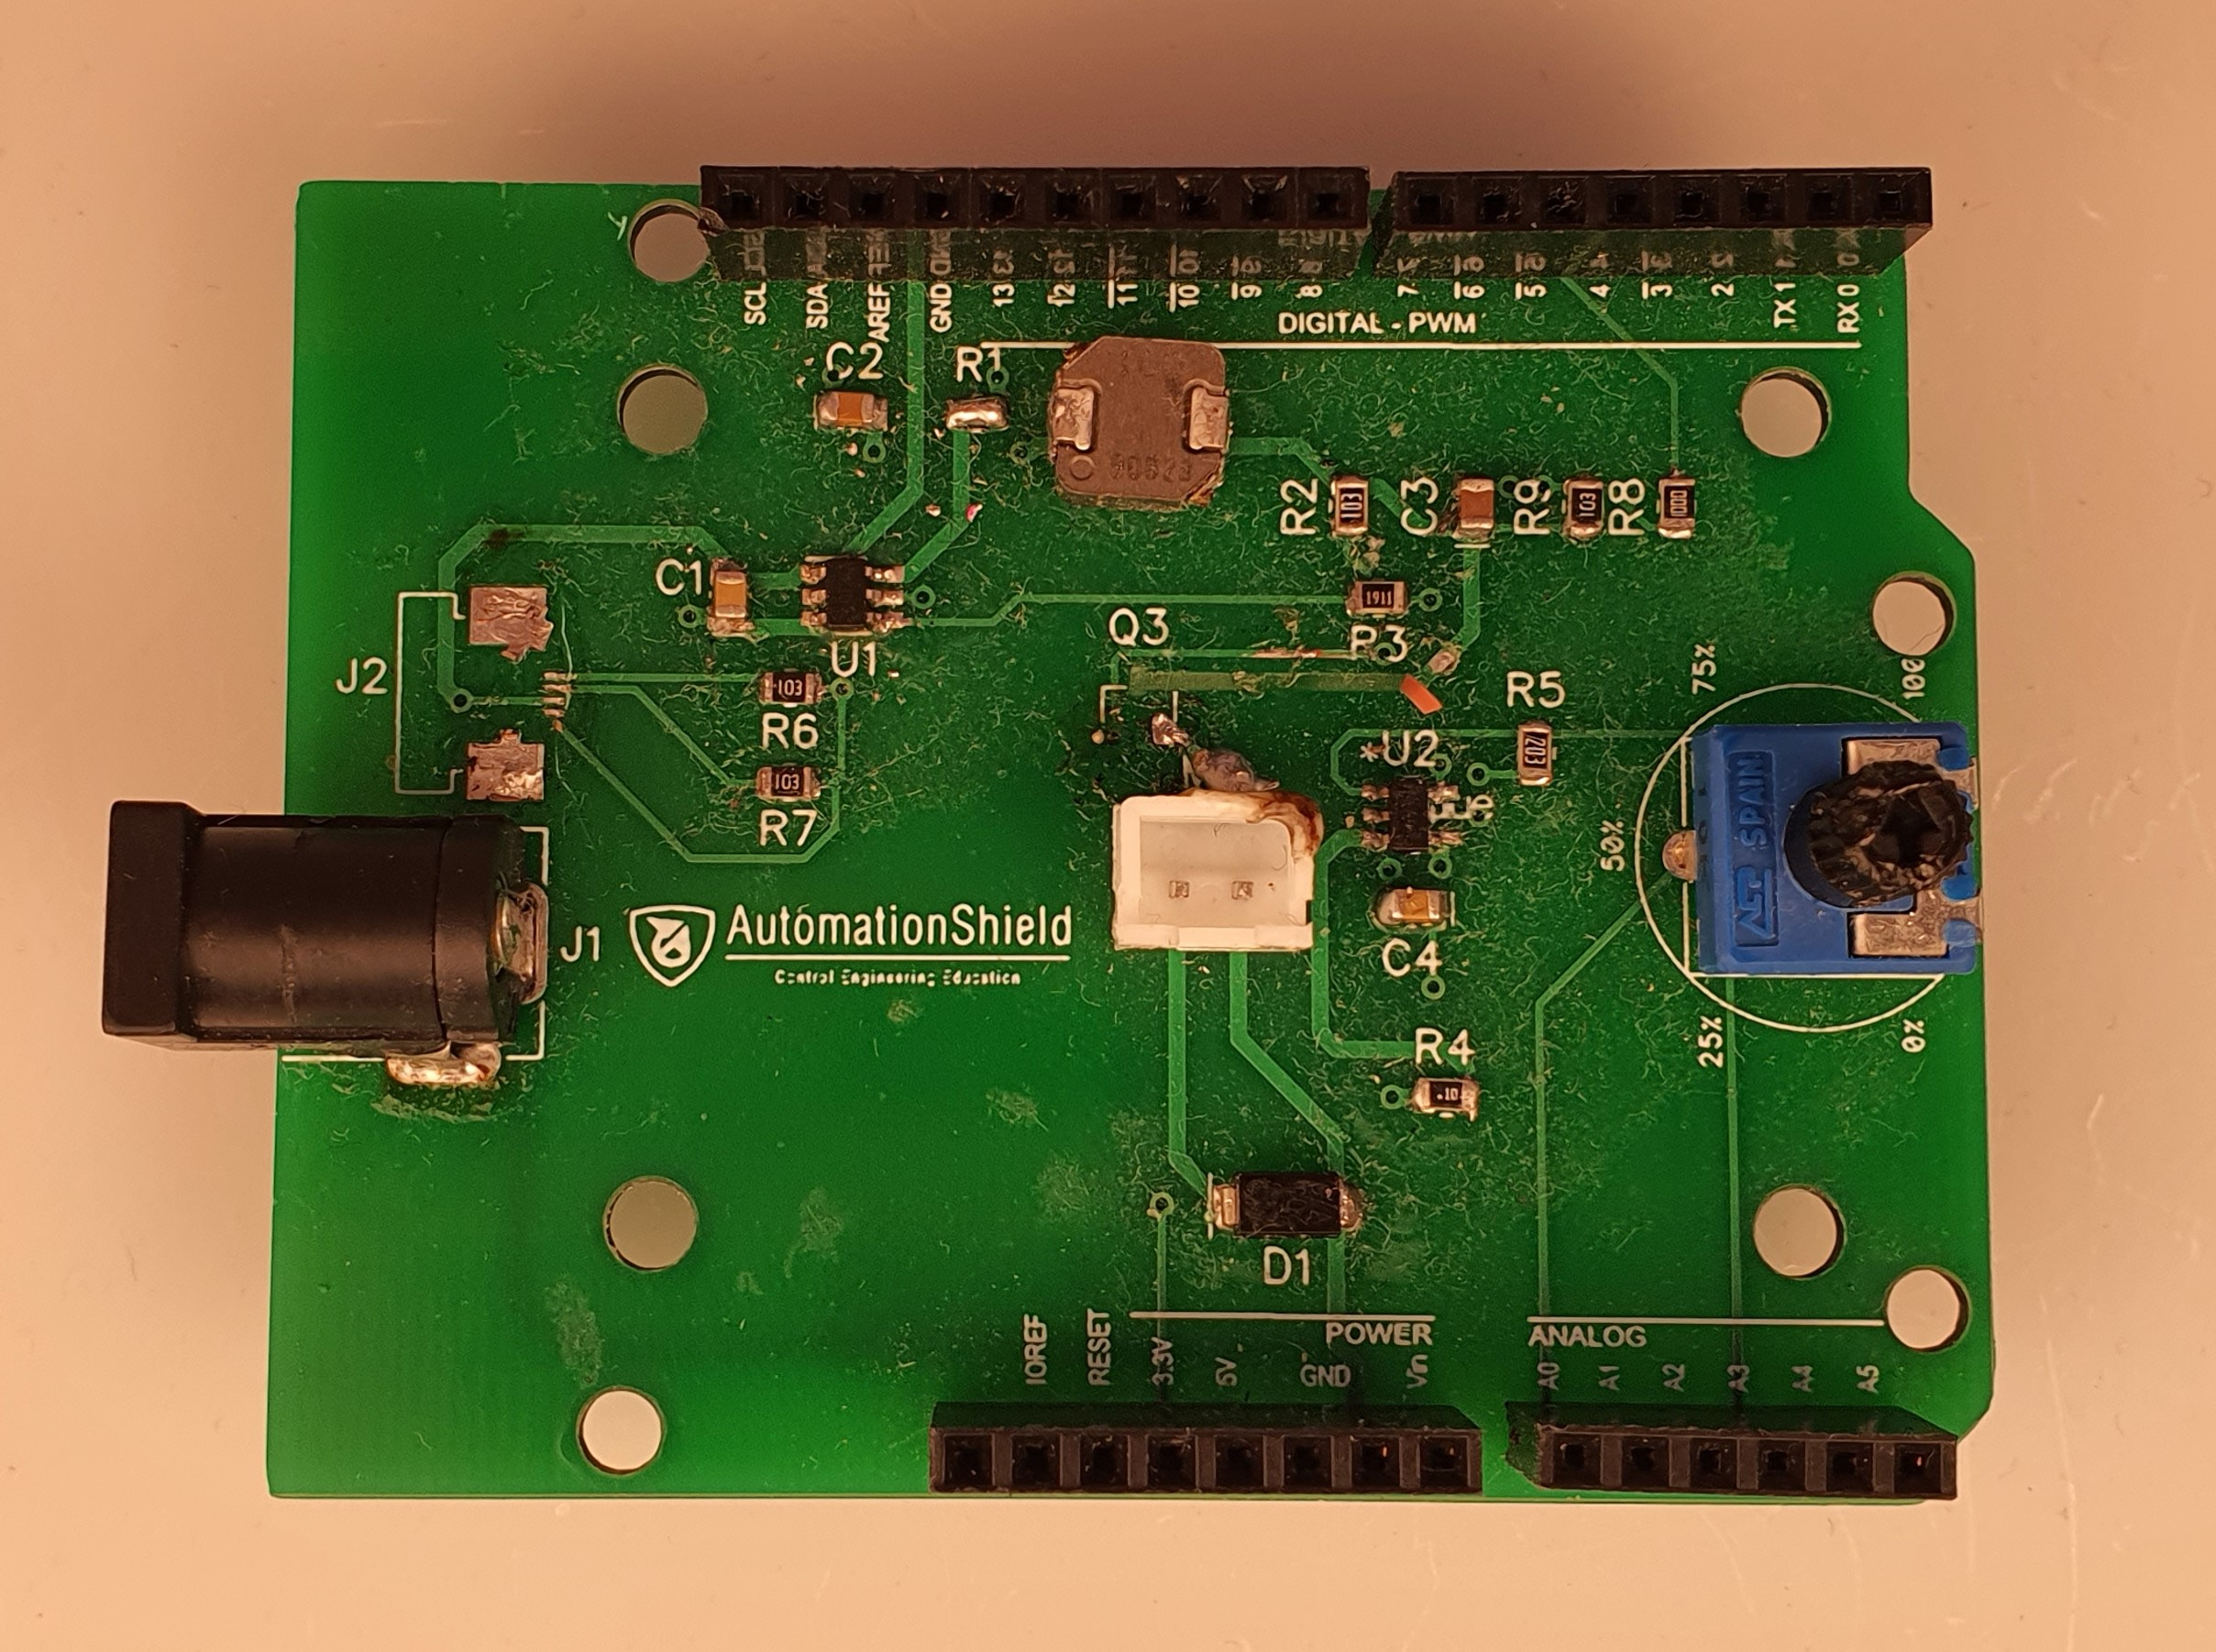
\includegraphics[width=80mm]{obr/oldshield.jpg}

(a)
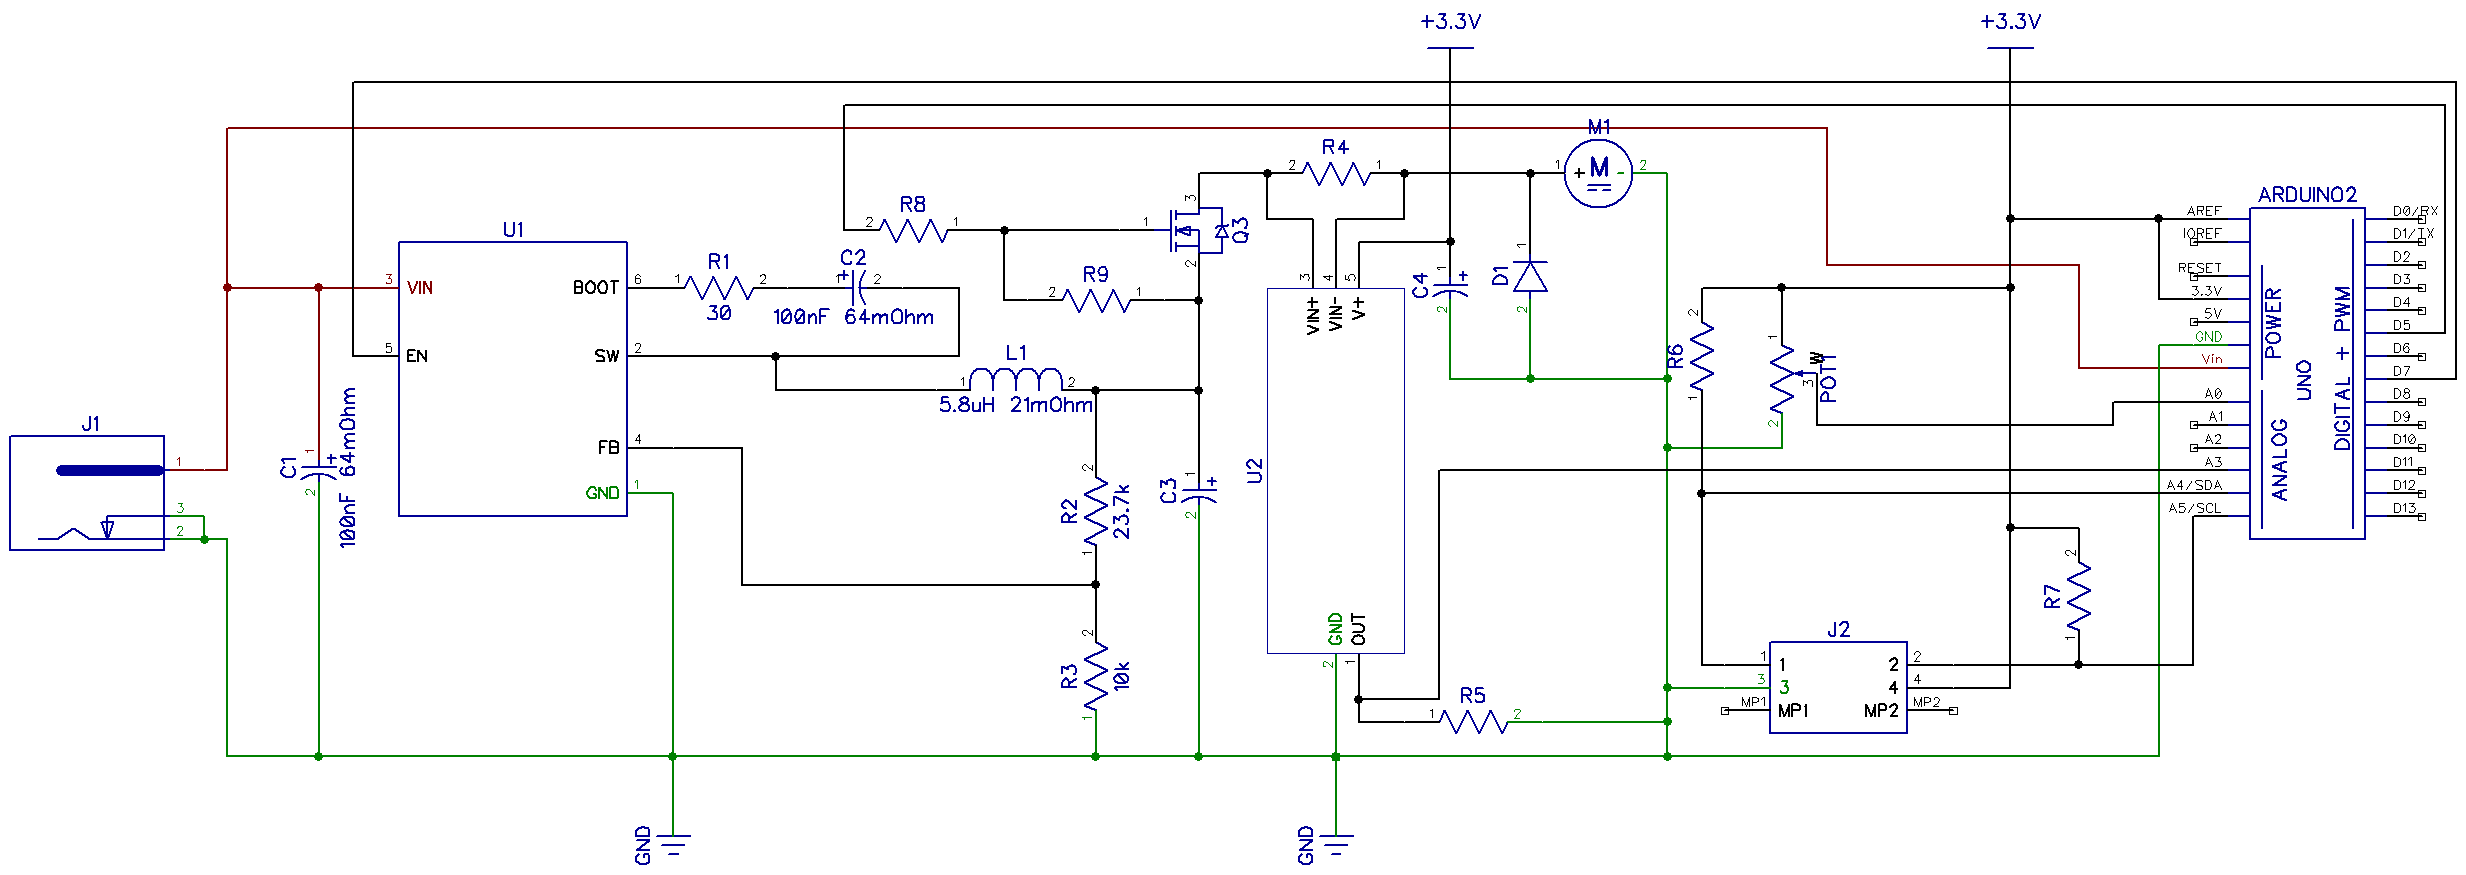
\includegraphics[width=\linewidth]{obr/oldshieldscheme.png}
(b)
\caption{(a) Prvá verzia AeroShieldu. (b) Schéma zapojenia prvej verzie AeroShieldu.}
\label{OBRAZOK 2.1.1}
\end{figure}

\vspace{3cm}

Prvá verzia dosky mala niekoľko nedostatkov, vďaka ktorým bola prakticky nepoužiteľná. Hlavnými nedostatkami boli:

\begin{itemize}
\item neprepojenie pinov komunikácie I2C tj. piny SDA a SCL senzoru hall efektu, ktorý slúži na meranie uhlu natočenia kyvadla,
\item nesprávne zapojenie mosfetu PMW45EN, ktorý ovláda PWM signál idúci do akčného člena,
\item nesprávne umiestnená ochranná dióda na konektoroch akčného člena,
\item nesprávne zapojený obvod s čipom INA169, ktorý slúži na meranie prúdu,
\item neprepojenie nulového konektora shieldu s nulovým konektorom arduina.
\end{itemize}

Základom tejto bakalárskej práce teda bolo najskôr pochopiť jednotlivé časti zapojenia, analizovať chyby a ich následná oprava. V rámci školského projektu bola vytvorená hlavná doska na ktorej sa nachádza väčšina elektroniky, avšak bola vytvorená aj verzia menšej dosky ktorá slúži na fungovanie senzoru hall efektu. Táto doska fungovala bezproblémovo a teda netrebalo nijakým spôsobom meniť jej schému zapojenia viditelnú na obr.\ref{OBRAZOK 2.1.2}.a. Tejto menšej doske sa budeme bližšie venovať v časti\ref{}, no jej podoba je viditelná na obr.\ref{OBRAZOK 2.1.2}.b.


\begin{figure}[!tbh]
\hfill
\subfigure[Schéma zapojenia externej dosky.]{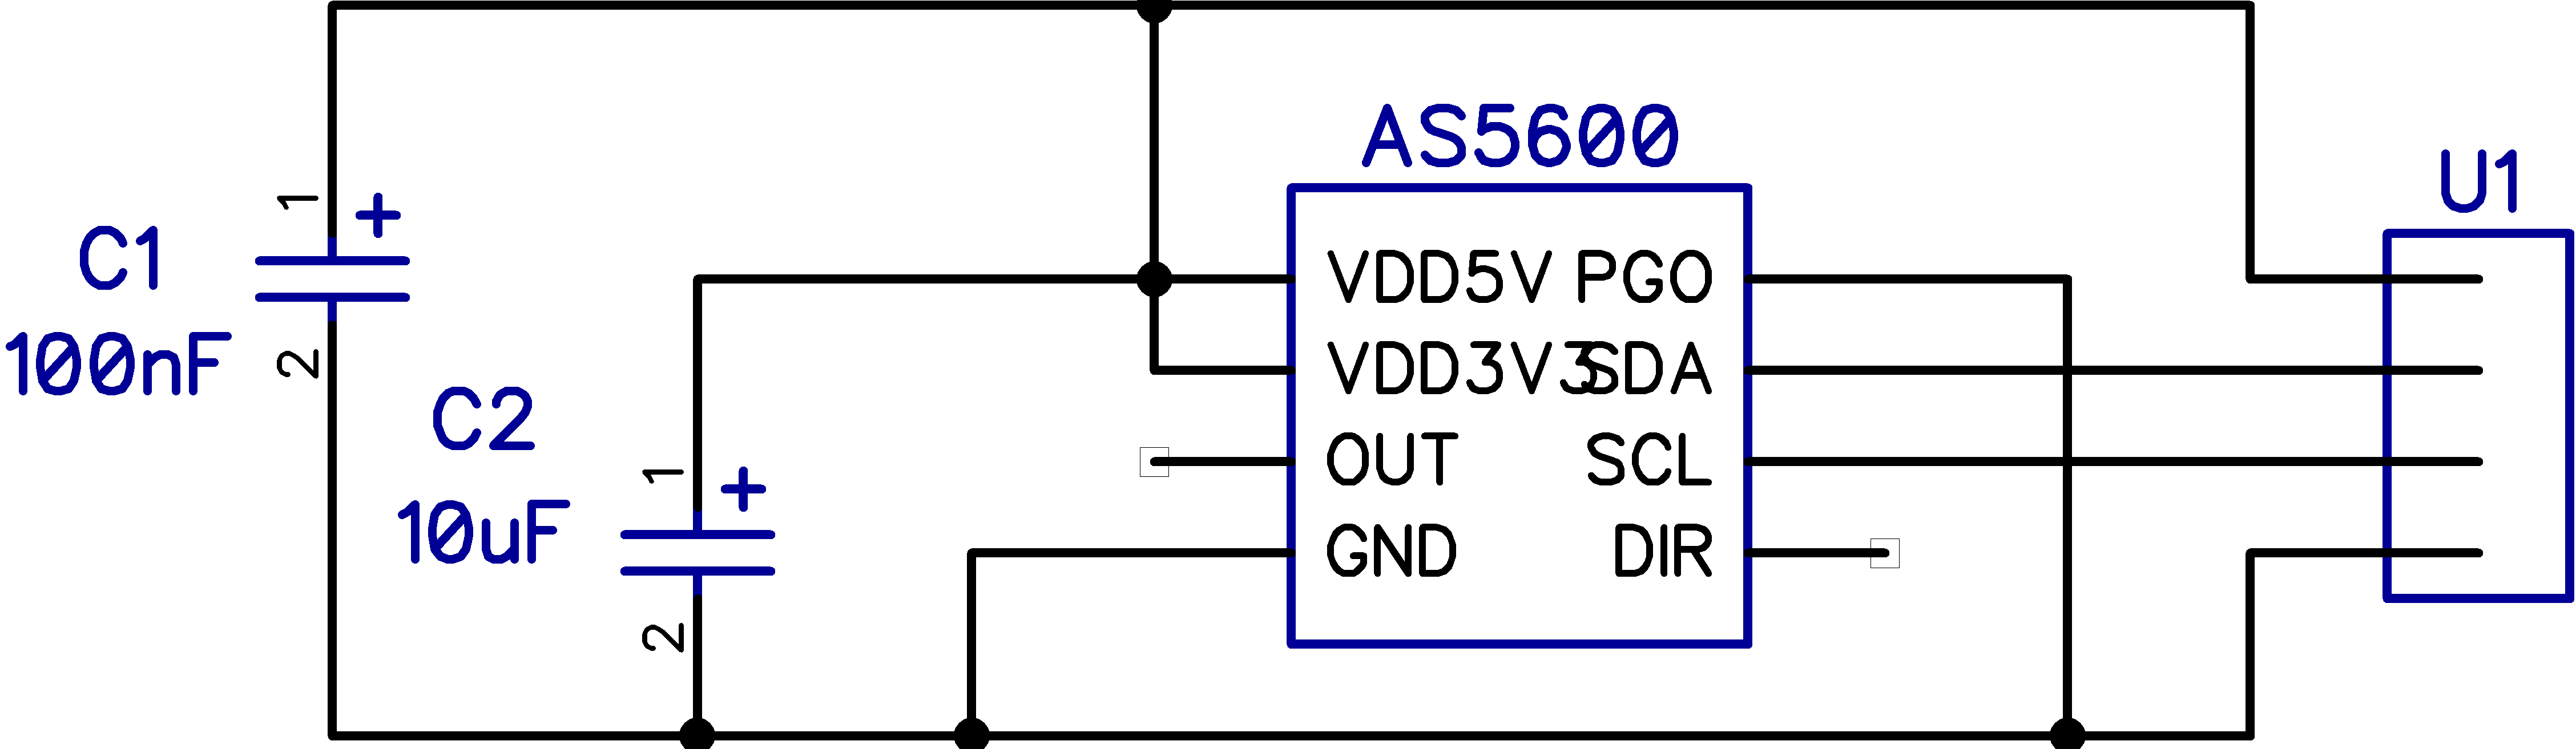
\includegraphics[width=9cm]{obr/as5600.png}}
\hfill
\subfigure[Doska slúžiaca na fungovanie senzoru hall efektu]{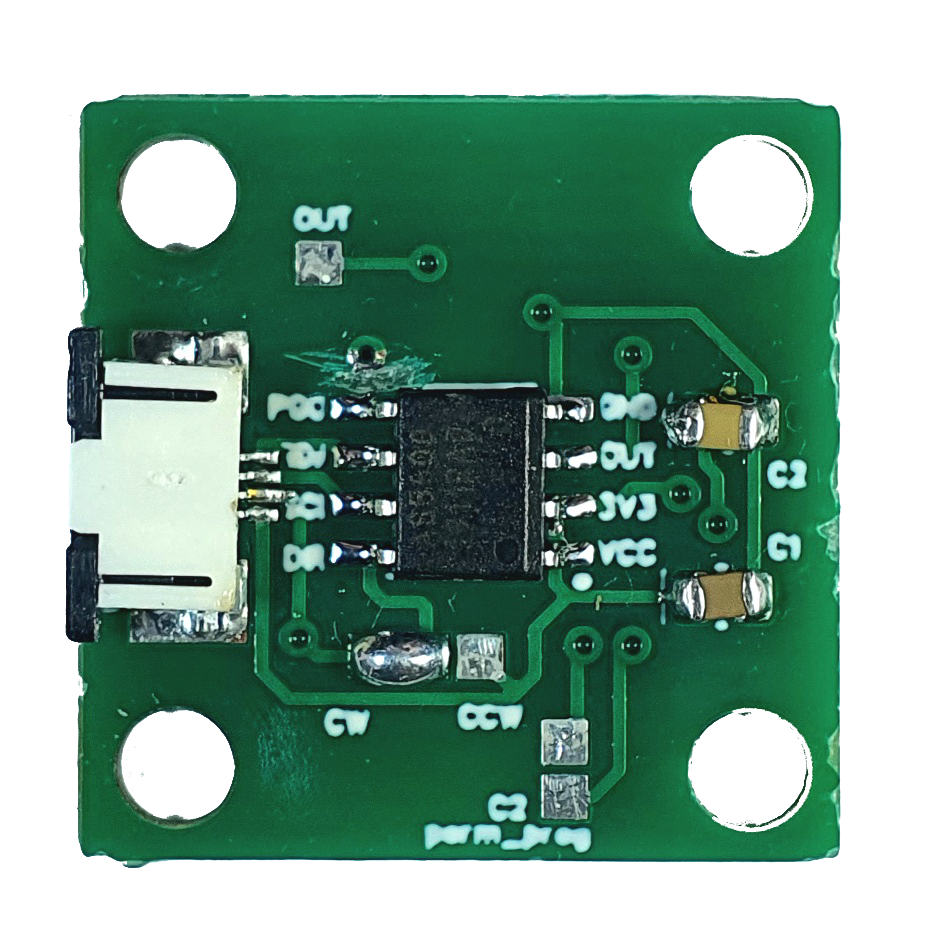
\includegraphics[width=5cm]{obr/fotoBreak.png}}
\hfill
\caption{meranie uhla kyvadla}\label{OBRAZOK 2.1.2}
\end{figure}

\vspace{3cm}


\section{Hardware}
\subsection{Popis súčiastok}

V tejto časti sa bližsie pozrieme na jednotlivé nevyhnutné súčasti zapojenia AeroShieldu. Konkrétne sa jedná o tieto prvky:
\begin{multicols}{2}
\begin{itemize}
\item napájanie
\item ovládanie akčného člena
\item meranie uhla natočenia kyvadla
\item meranie prúdu
    \end{itemize}
    \end{multicols}


\subsubsection{Znižovanie napätia}
\label{nap}

Na správne napájanie akčného člena, motorčeka, potrebujeme napätie v rozmedzí 0-3,7V. Na shield je však privázdané, pomocou koaxiálneho napájacieho konektora, napätie 12V ktoré by motor v priebehu chvíle zničilo. Potrebujeme preto spôsob ako znížiť privádzané napätie, no súčastne neznížiť privádzaný prúd potrebný na pohon motorčeka. Na tieto účely slúži takzvaný buck converter alebo konvertor na zníženie napätia. Hlavnou Časťou konvertora je čip TPS56339 od výrobcu Texas Instruments obr.\ref{OBRAZOK 2.1}.b. Znižovanie napätia funguje za pomoci dvoch integrovaných N-kanálových 70-m$\Omega$ a 35-m$\Omega$ high-side mosfetov\footnote[4]{N-kanálový mosfet je typ mosfetu, v ktorom tok prúdu nastáva kvôli pohybujucím sa, záporne nabitým elektrónom. "High-side" znamená, že prúd prechádza z napájania, cez mosfet do záťaže a potom do zeme} a dalších komponentov. Celkový prevádzkový prúd zariadenia je približne 98$\upmu$A, keď funguje bez spínania a bez záťaže. Keď je zariadenie vypnuté, napájací prúd je približne 3$\upmu$A a zariadenie umožňuje nepretržitý výstupný prúd do 3 A\cite{buckobr}.

\begin{figure}[!tbh]
\hfill
\subfigure[Schéma zapojenia konvertora napätia.]{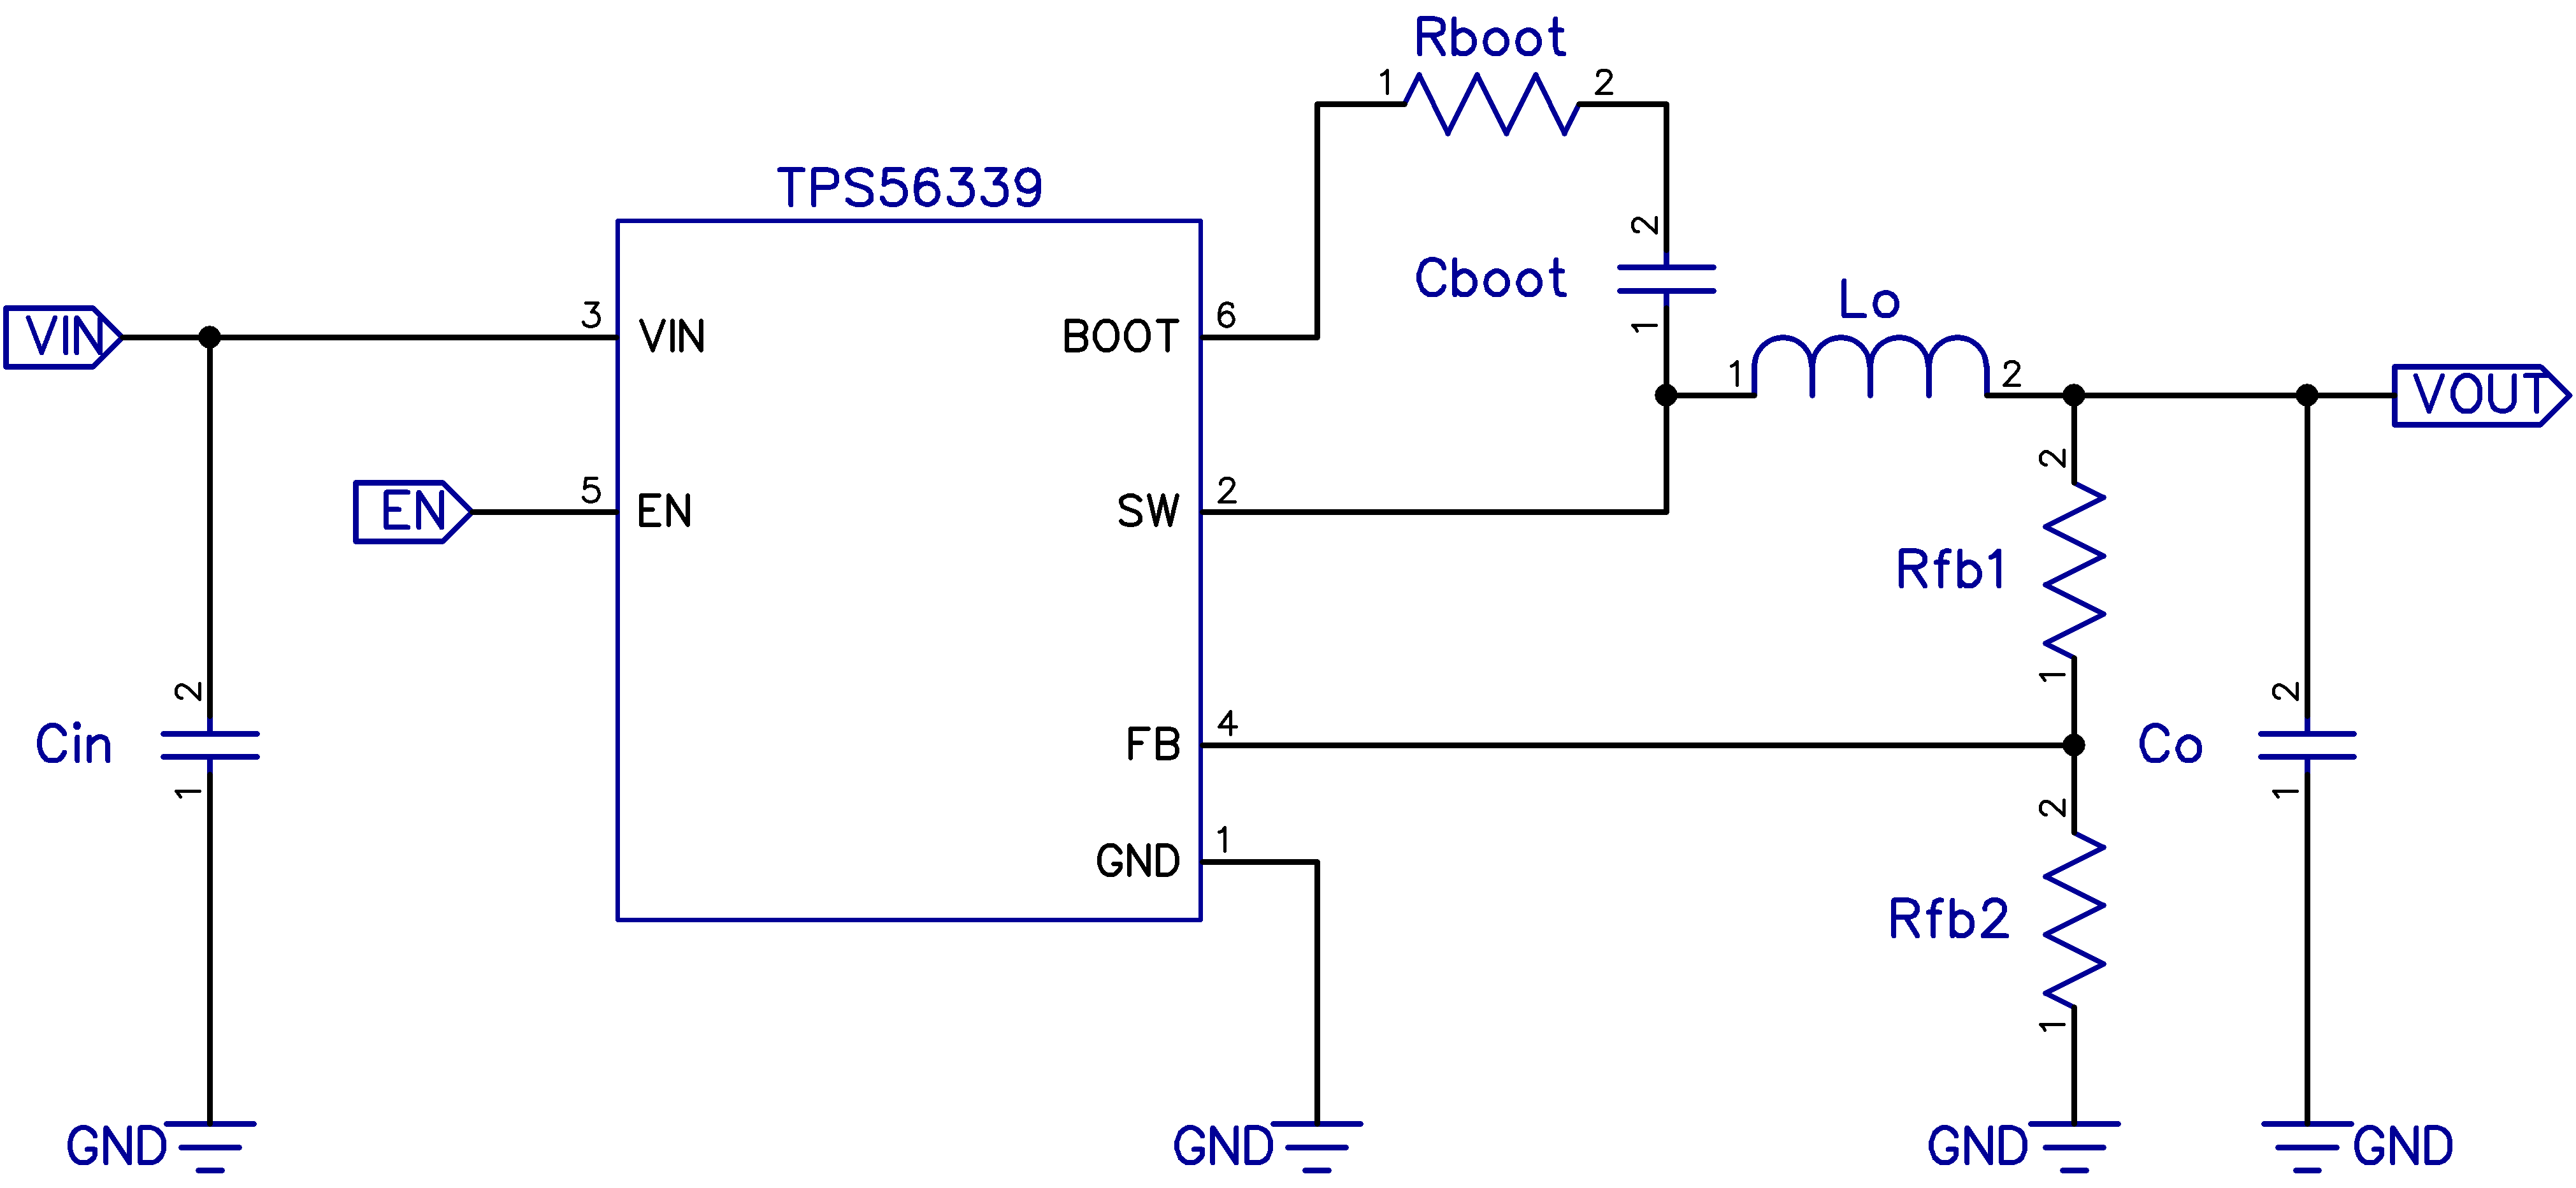
\includegraphics[width=9cm]{obr/schemaBuck.png}}
\hfill
\subfigure[{čip TPS56339\cite{buckobr}}]{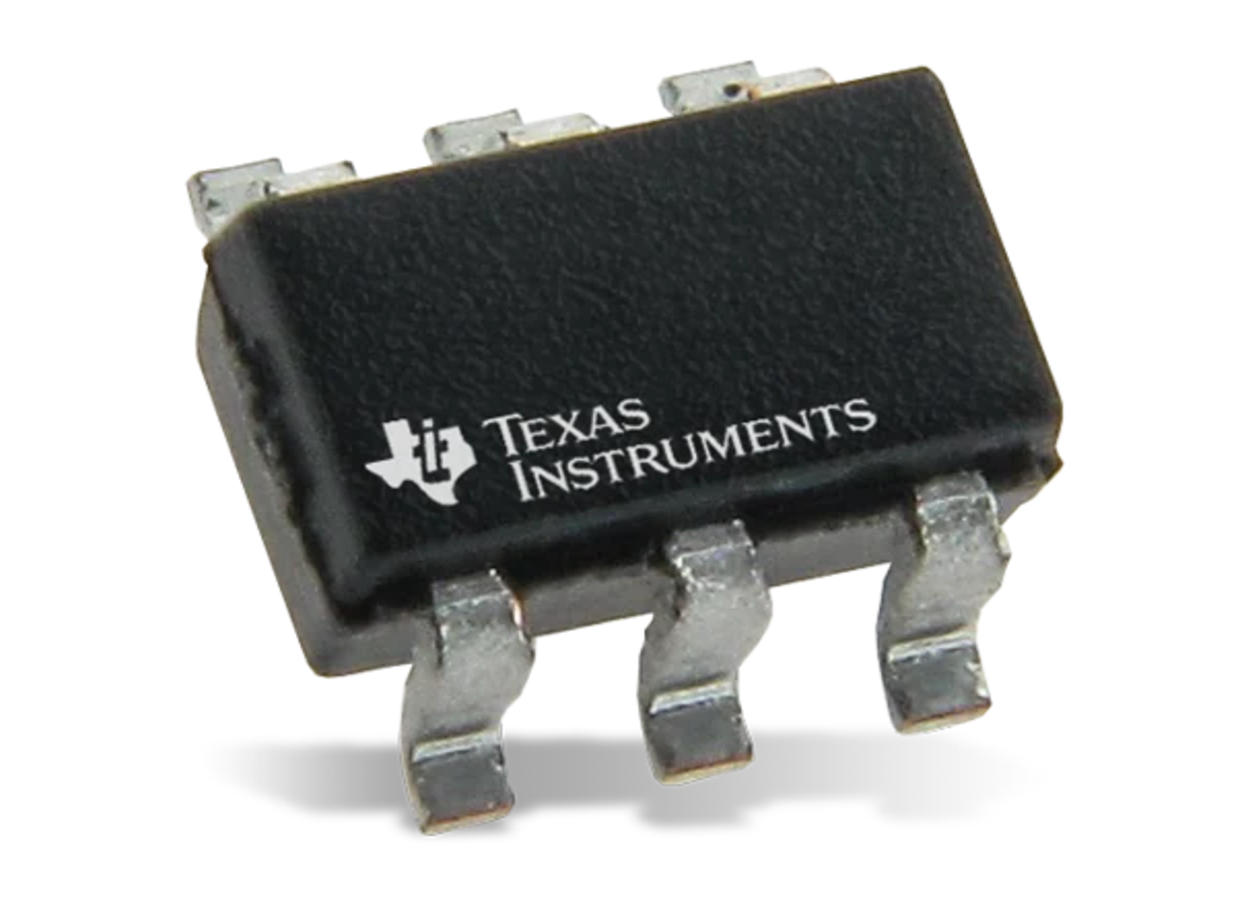
\includegraphics[width=5cm]{obr/cip.eps}}
\hfill
\caption{buck converter}\label{OBRAZOK 2.1}
\end{figure}

 Na čip je privádzané napätie 12V ktoré sa pomocou zapojenia, vididelného na schéme obr.\ref{OBRAZOK 2.1}.a, znižuje na napätie 3,7V. Napájanie motora musí byť realizované externe pomocou koaxiálneho napájacieho konektora, z dôvodu vysokého prúdu odoberaného motorom počas vysokého zaťaženia. Rovnaký konektor sa síce nachádza aj na doske Arduino UNO a pomocou VIN pinu sa dajú napájať napätím 0-12V aj iné zariadenia, avšak tento pin je napojený na diódu obmedzujúcu prúd na 1A\cite{ampere}\cite{ampere2}.



\subsubsection{akčný člen}
\label{akcclen}

Ako akčný člen AeroShieldu je použitý 7mm, 3,7V motorček na jednosmerný prúd, bez jadra. “coreless motor“ alebo motor bez jadra je motor s cievkou navinutou samou na sebe a nie na železe\cite{coreless}. Takéto jadro ale samé o sebe nie je veľmi pevné a nedrží dobre tvar, preto sa častokrát zalieva epoxidom. Stator je vyrobený z magnetov na báze vzácnych zemín, ako je neodým alebo SmCo(samárium-kobalt), ktoré sa nachádzajú vo vnútri bezjadrového rotora.

Takýto motor ponúka mnoho výhod oproti motoru so železným jadrom. Tým že jadro v sebe nemá železo, výrazne sa znižuje hmotnosť a tým aj zotrvačnosť rotora, čo je dôležité pre naše použitie kedy potrebujeme dosahovať vysokú akceleráciu a rýchle spomalenie rotora. Ďalšou výhodou je fakt že nedochádza k stratám na železe a tým pádom sa účinnosť takýchto motorov blíži až ku 90\%-\cite{5545147}. Motor resp. otáčky motora sú riadené pomocou impulzovej šírkovej modulácie(PWM) a tieto impulzy do motoru prechádzajú cez N-kanálový mosfet PMV45EN2 od výrobcu Nexperia\cite{pmv}.



\begin{figure}[!tbh]
\hfill
\subfigure[Schéma zapojenia motorčeka.]{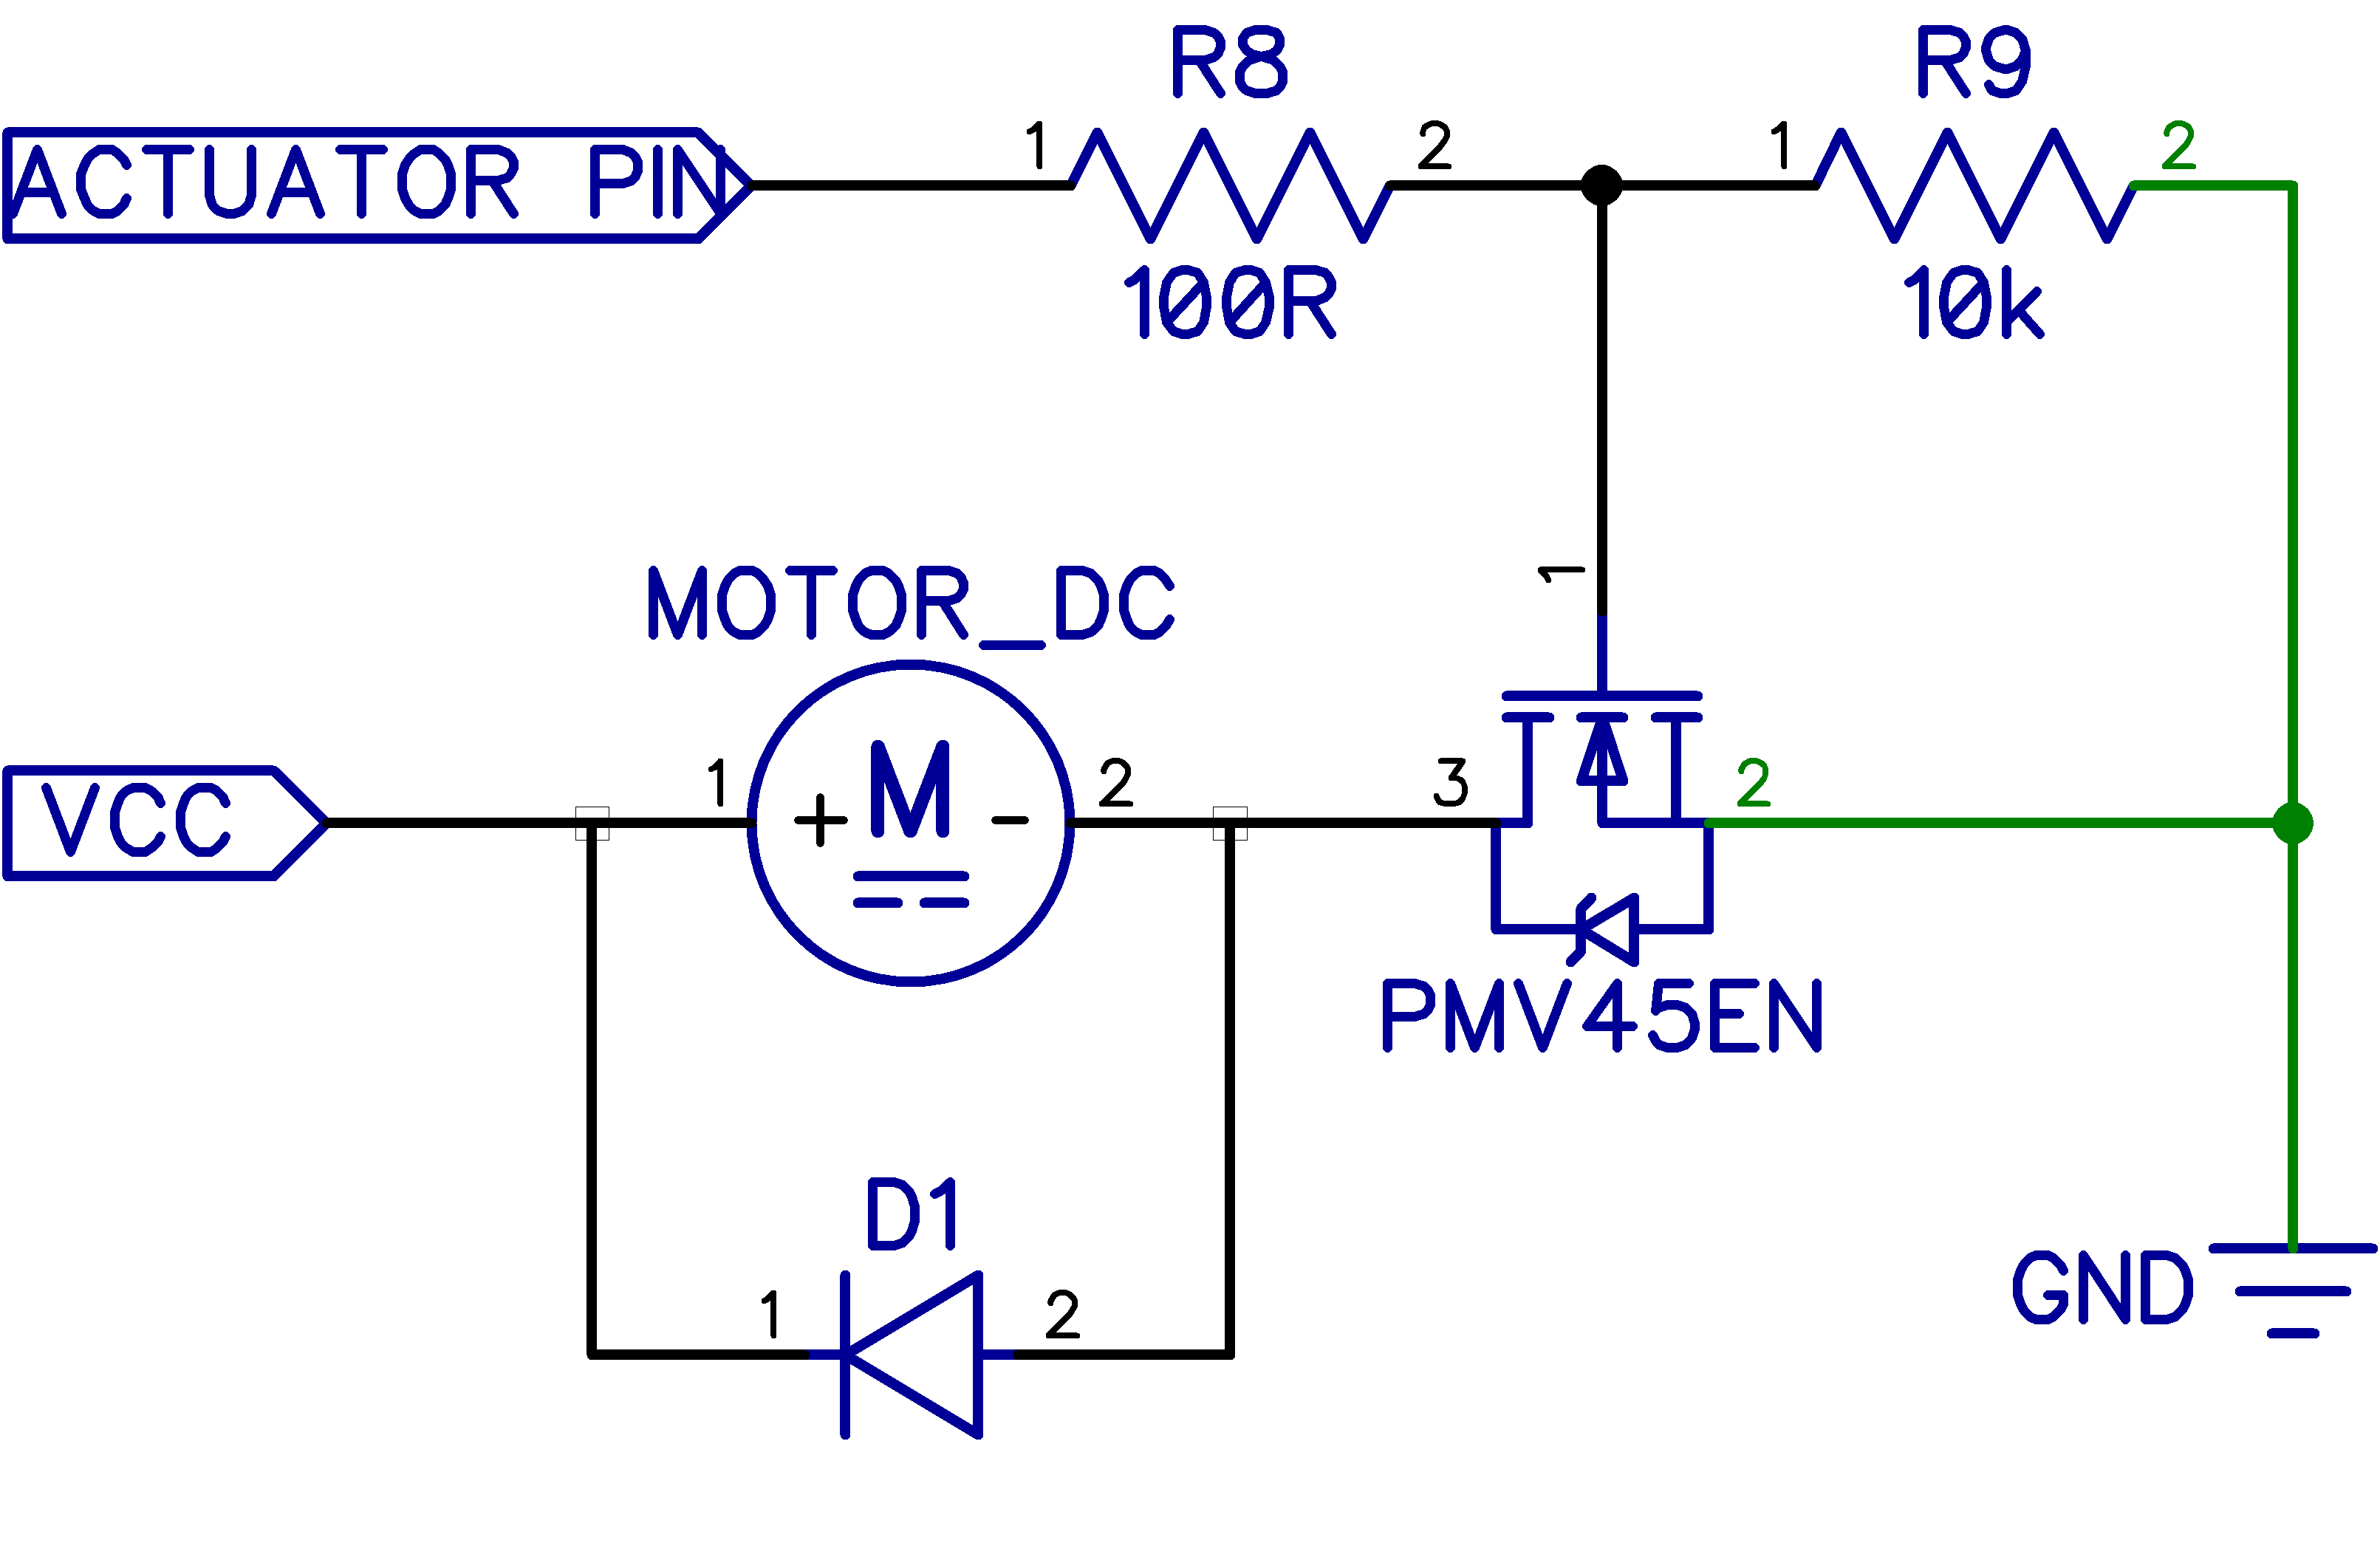
\includegraphics[width=7cm]{obr/MotorScheme.png}}
\hfill
\subfigure[{Motorček\cite{corelessMotor}}]{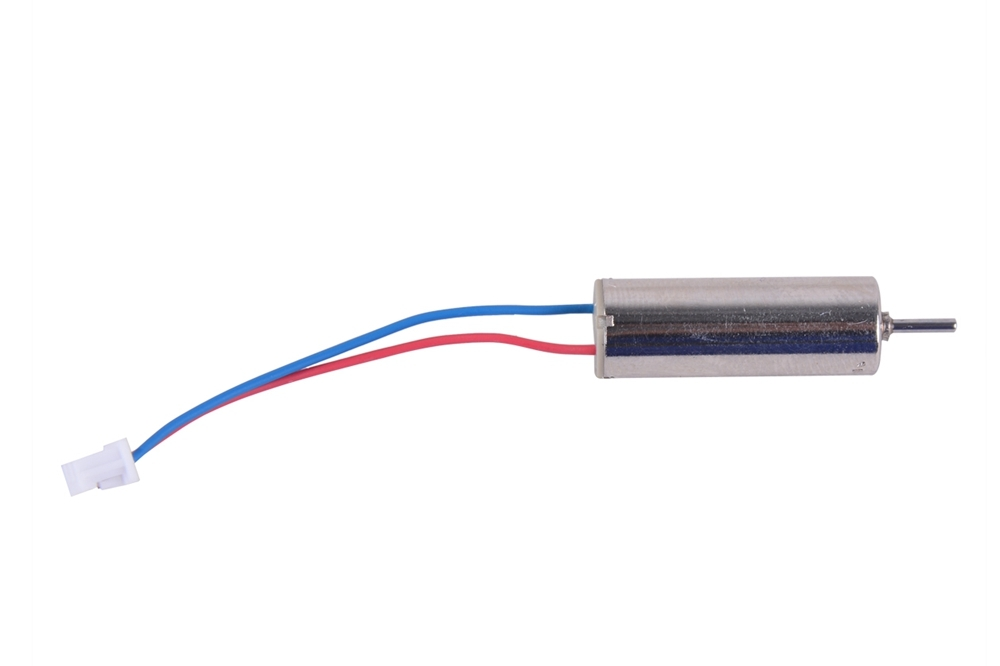
\includegraphics[width=7cm]{obr/coreless.jpg}}
\hfill
\caption{akčný člen}\label{OBRAZOK 2.3}
\end{figure}


\subsubsection{meranie prúdu}
\label{merprud}

Pre čo najpresnejšie ovládanie akčného člena sústavy, motora, je dobré vedieť nie len napätie, ktorým je motor ovládaný, ale aj prúd, ktorý motor odoberá. Na tieto účely sa používajú monitory prúdu, takzvané "current shunt monitors". V AeroShielde je použitý snímač INA169NA/250 od výrobcu Texas Instruments obr.\ref{OBRAZOK 2.3}.b.

INA169 funguje na základe zaznamenávania zmien napätia na stranách shunt rezistora obr.\ref{OBRAZOK 2.3}.a. Na základe nameraného úbytku napätia, vysiela senzor poďla nami zvoleného stupňa zosilnenia, prúd, ktorý je ďalej pomocou rezistoru $R_{l}$ premenený na napätie s maximálnou hodnotou $V_{OUTMAX} = V_{IN-} - 0.5V $.

 Prúd $I_{s}$ odoberaný motorom, vypočítame pomocou vzorca $I_{s} = \dfrac{V_{OUT}\: x \: 1k\Omega}{R_{s} \: x \: R_{l}} $ kde $V_{OUT}$ je napätie namerané na výstupe, 1k$\Omega$ je konštanta vnútorných odporov senzoru, $R_{s}$ je hodnota shunt rezistora v $\Omega$ a $R_{l}$ je hodnota rezistora na výstupe, taktiež v $\Omega$\cite{INA}.

\begin{figure}[!tbh]
\hfill
\subfigure[Schéma zapojenia snímača prúdu.]{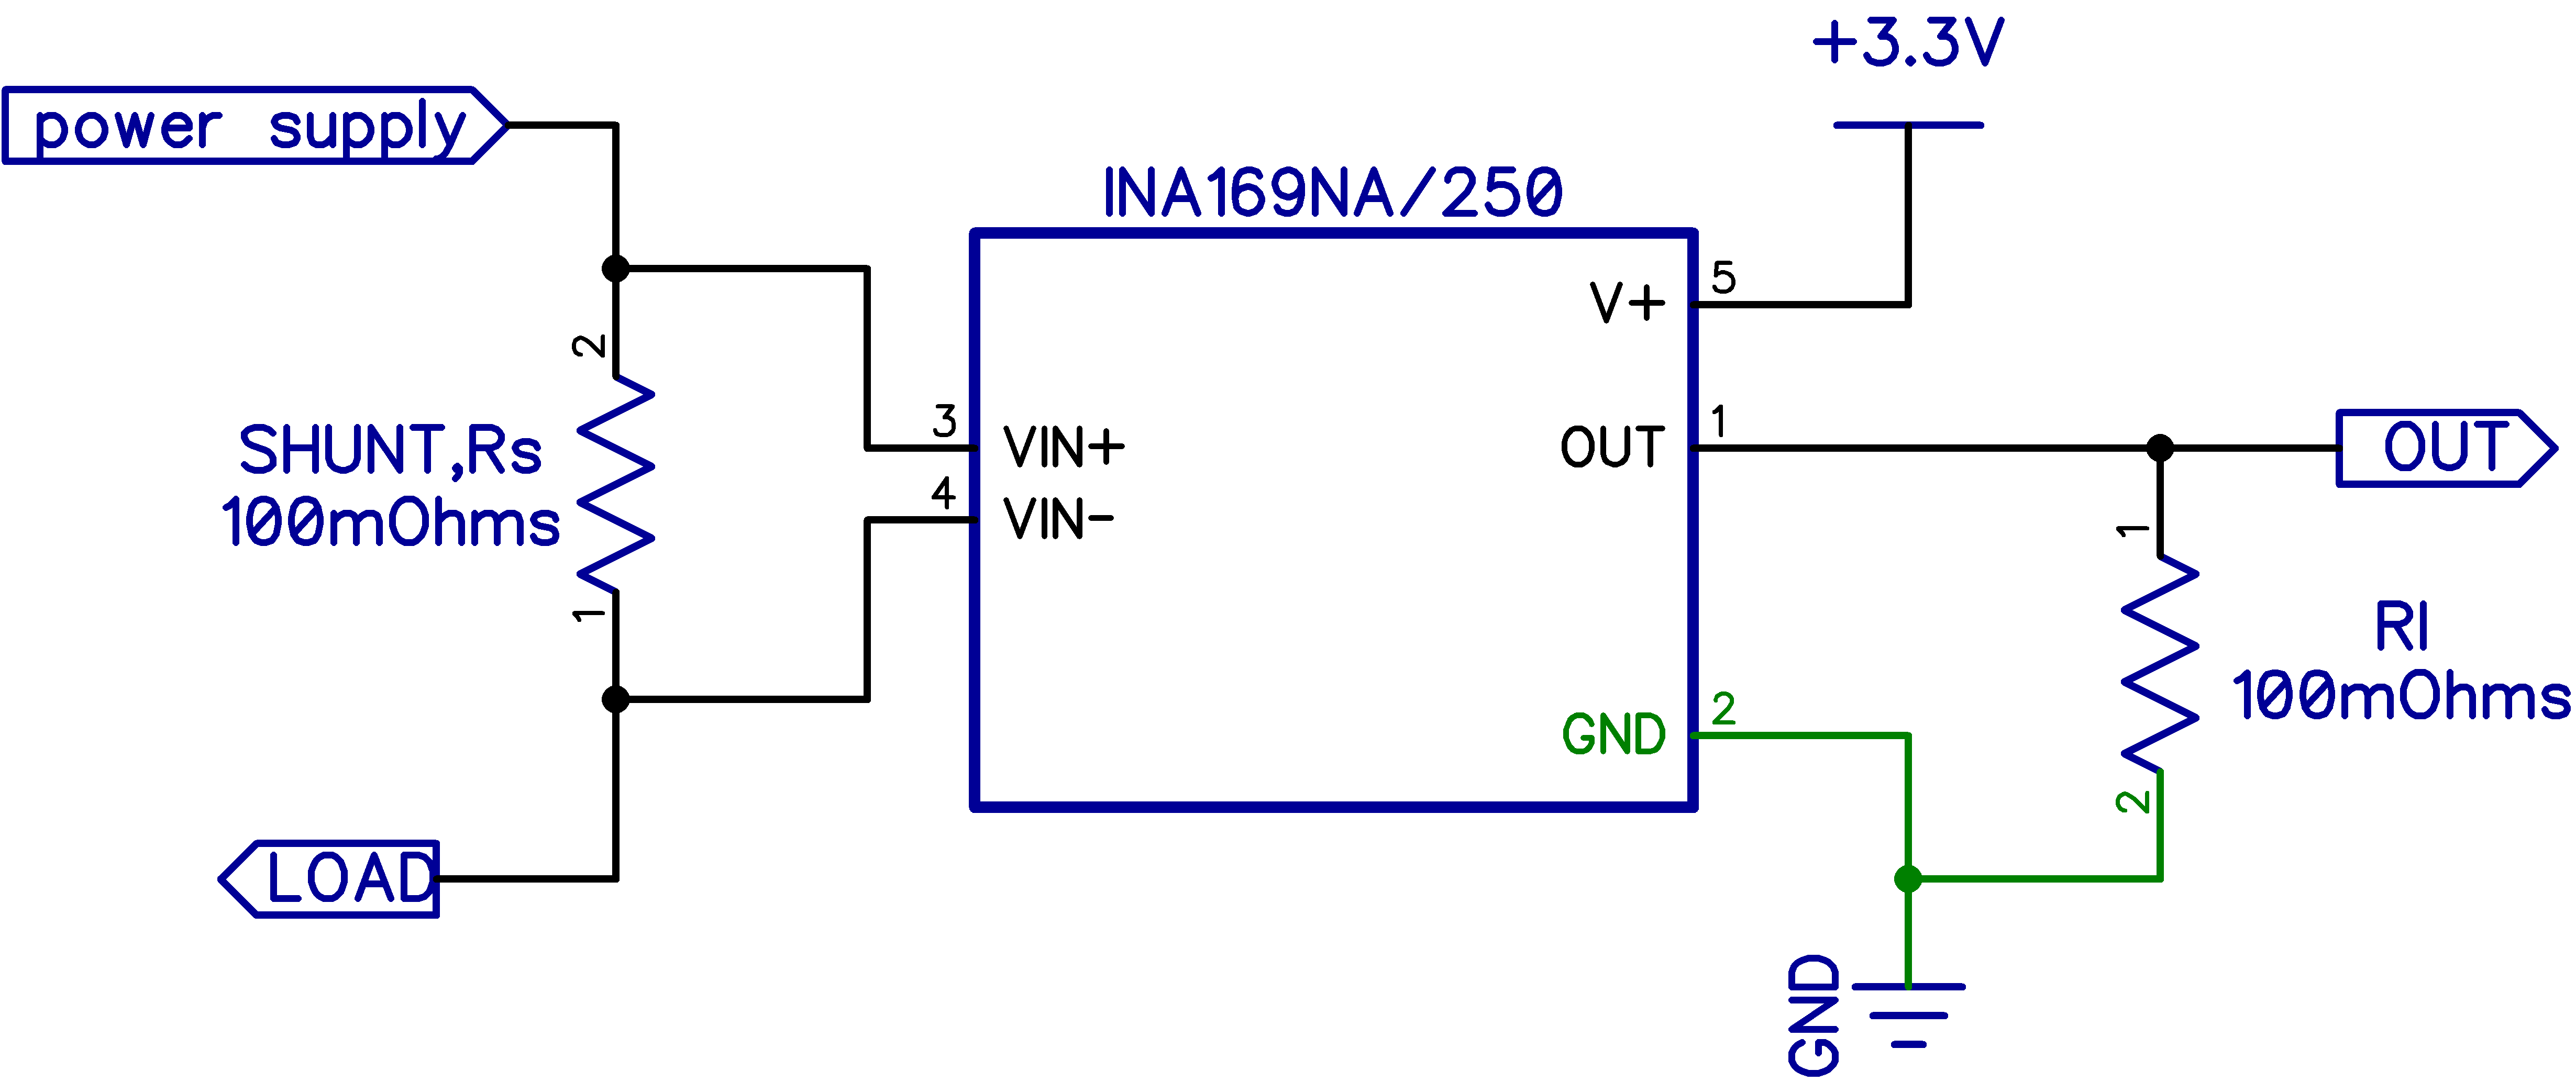
\includegraphics[width=9cm]{obr/INAschema.png}}
\hfill
\subfigure[{Senzor INA169NA/250\cite{INAobr}}]{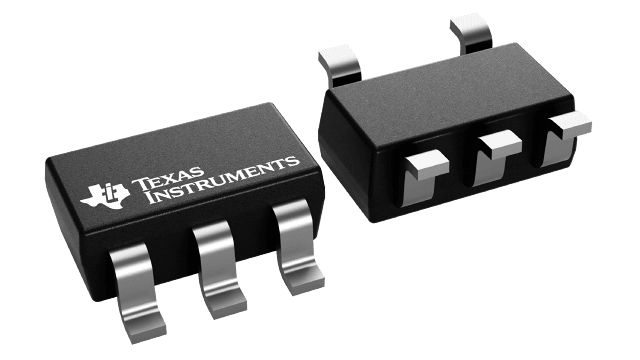
\includegraphics[width=6cm]{obr/ina.png}}
\hfill
\caption{meranie prúdu}\label{OBRAZOK 2.3}
\end{figure}


\label{Hall}
\pagebreak

\subsubsection{meranie uhla kyvadla}
\label{meruhl}

Na správne fungovanie AeroShieldu je dôležité vedieť s vysokou presnosťou merať uhol naklonenia kyvadla. Na tento účel sme si zvolili meranie uhlu bezkontaktnou formou, pomocou snímača na princípe hallovho javu. Hallov jav vieme opísať ako vznik priečneho elektrického poľa v pevnom materiáli, keď ním preteká elektrický prúd a tento materiál je umiestnený v magnetickom poli, ktoré je kolmé na prúd\cite{Hall}. Toto elektrické pole resp. vznik elektrického potenciálu vieme detegovať a na základe jeho zmeny vieme určit rotáciu kyvadla. V kyvadle je na konci horizontálneho ramena umiestnený špeciálny magnet kruhového tvaru ktorý je polarizovaný naprieč prierezom magnetu.

Ako senzor na meranie hallovho efektu je použitý AS5600 od výrobcu OSRAM obr.\ref{OBRAZOK 2.2}.b. Signály prichádzajúce zo snímača sa najprv zosilnia, následne sú filtrované a prechádzajú konverziou pomocou analógovo-digitálneho prevodníkom (ADC). Snímaná je aj intenzita magnetického poľa, ktorá sa ďalej používa na
automatické riadenie zosilnenia(AGC), ktoré slúži na kompenzáciu teploty a veľkosti magnetického poľa.

Na výber sú dva typy výstupu a to analógový výstup alebo digitálny výstup s kódovaním PWM. Senzor má taktiež aj možnosti interného programovania pomocou rozhrania I2C.
V našom prípade používame 12-bitový analógový výstup s rozlíšením 0°5'16". Toto rozlíšenie nám umožnuje s vysokou presnosťou kontrolovať naklonenie kyvadla a na základe získaných informácii ovplyvňovať fungovanie akčného členu sústavy. Schéma zapojenia čipu na meranie uhlu môžeme vidieť na obr.\ref{OBRAZOK 2.2}.a.



\begin{figure}[!tbh]
\hfill
\subfigure[Schéma zapojenia čipu na meranie uhlu.]{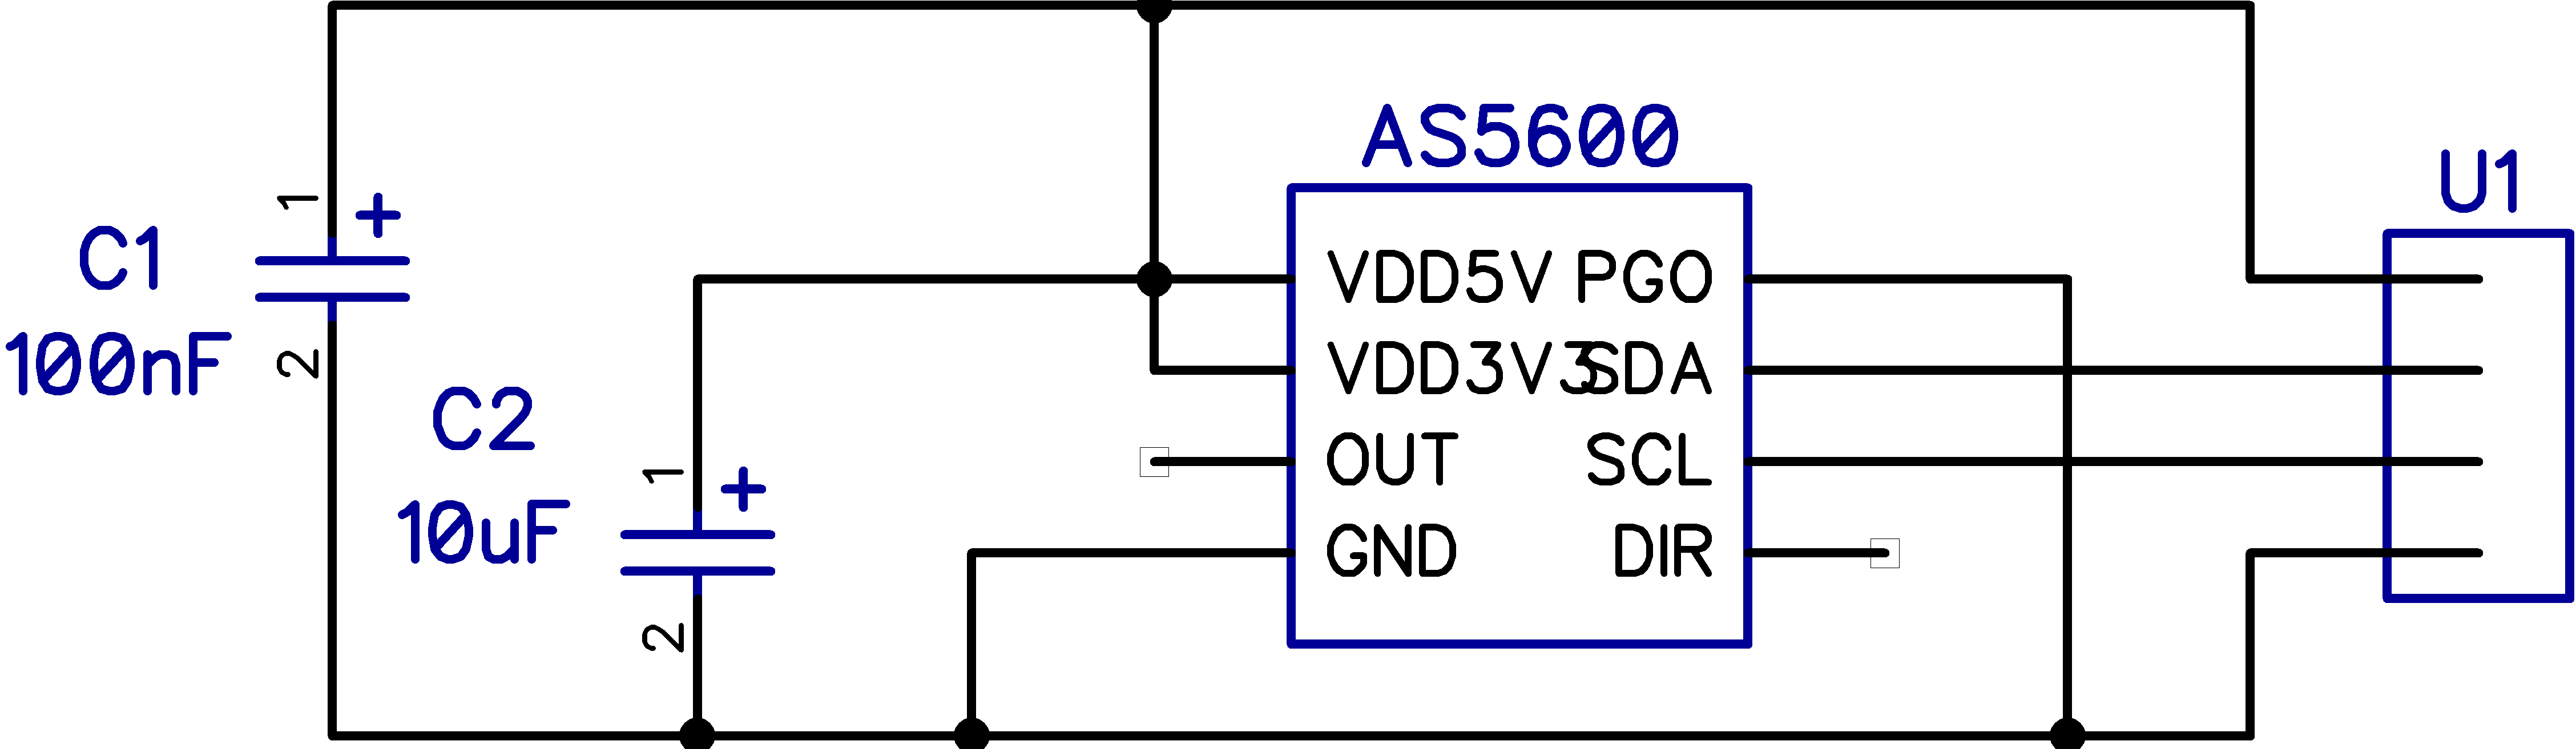
\includegraphics[width=10cm]{obr/as5600.png}}
\hfill
\subfigure[{čip AS5600\cite{As5600obr}}]{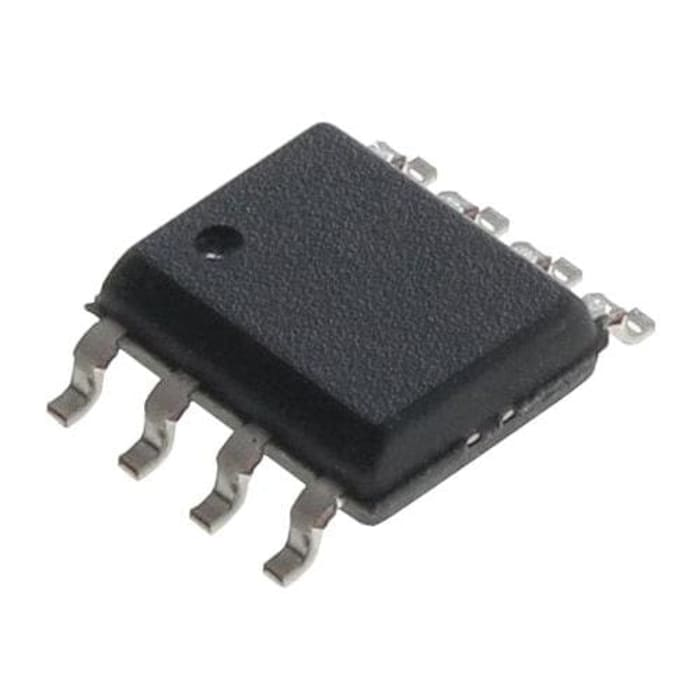
\includegraphics[width=4cm]{obr/hall.jpg}}
\hfill
\caption{meranie uhla kyvadla}\label{OBRAZOK 2.2}
\end{figure}

\newpage


\subsection{Schéma zapojenia}

Všetky schémy zapojenia boli tvorené v bezplatnej verzii programu DipTrace. DipTrace slúži ako prostredie na tvorbu elektrotechnických schém, potrebných pre výrobu dosiek plošných spojov, ako aj pre účely prehľadnosti zapojenia komponentov na týchto doskách. Program v sebe zahŕňa časť pre tvorbu samotných komponentov, pokial sa tieto už nenachádzajú v niektorej z knižníc programu, časť kde sa tvoria schémy zapojenia a časť na tvorbu dosiek plošných spojov.

Nie všetky komponenty potrebné na tvorbu AeroShieldu boli zahrnuté v knižniciach DipTracu, avšak tieto komponenty sa nachádzali na stiahnutie na stránkach výrobcov odkiaľ boli importované do novej knižnice, slúžiacej na účely tvorby schémy AeroShieldu. Do programu bola taktiež vložená knižnica AutomationShieldu ktorá má v sebe najčastejšie používané komponenty. Pri tvorbe schémy zapojenia sa najskôr všetky potrebné komponenty umiestnia na štvorčekovú plochu a približne sa určí ích poloha. Jednotlivé komponenty majú podobu elektrotechnických značiek a každý komponent má ku sebe priradené reálne vlastnosti daného dielu(veľkosť, zapojenie, dĺžka pinov a iné).

Polohu volíme takú, aby schéma bola čo najprehladnejšia a komponenty ktoré sú medzi sebou prepojené, boli čo najbližšie pri sebe. Akonáhle máme všetky komponenty uložené začneme s ich postupným prepájaním. Pri zapájaní jednotlivých komponentov sa riadime katalógovými listami jednotlivých komponentov, v ktorých býva zväčša aj návrh ich zapojenia.

Veľmi dobrou vlastnosťou pogramu DipTrace je možnosť zafarbovania jednotlivých elektrických spojení, rozličnými farbami a názvami. Tento fakt nám veľmi uľahčuje na prvý pohľad rozoznať napríklad elektrické spojenia zeme- 0V zelená, fázové spojenia- 3,3V červená obr.\ref{OBRAZOK 2.3}. Na schéme zapojenia môžeme vidieť všetky komponenty, potrebné na správne fungovanie AeroShieldu. Názvy komponentov sú uvádzané základnými značkami
\begin{multicols}{3}
    \begin{itemize}
\item R- Rezistor
\item C- Kapacitor
\item J- Konektor
\item U- Mikročip
\item L- Cievka
\item D- Dióda
\item M- Motor
    \end{itemize}
    \end{multicols}


\begin{figure}[!tbh]
\includegraphics[width=\textwidth]{obr/aeroSchema.png}
\caption{Schéma zapojenia AeroShieldu}\label{OBRAZOK 2.3}
\end{figure}

\subsection{Doska plošných spojov}

Po návrhu a kontrole schém zapojenia sa schémy dalej spracovávajú do podoby dosky plošných spojov. Schémy exportujeme do programu DipTrace PCB v ktorom máme následne niekoľko možností postupu. Jednotlivé komponenty sa nám už zobrazujú v reálnej podobe, takže vidíme ich veľkosť a rozmiestnenie pinov na pájkovanie. Dosky plošných spojov majú niekoľko nevýhod, ale aj výhod oproti ponúkaným alternatívam\cite{dosky}. 

Výhodou je fakt, že vodivé spojenia medzi jednotlivými súčiastkami zapojenia, sú realizované vrstvou medi ktorá je ukrytá pod ochrannými vrstavmi povrchu dosky, narozdiel od typických káblových spojení. Káble majú niekoľko nedostatkov ako to že sa vedia ľahko vypojiť, ľahko dochádza k ich porušeniu a v neposlednom rade, nepôsobia veľmi esteticky. V prípade nesprávneho prepojenia pinov má jednodoznačnú výhodu spoj realizovaný káblami, kedže pri doskách plošných spojov sa s už hotovými cestami manipuluje obtiažne. Ďaľšou výhodou dosiek plošných spojov je skutočnosť, že sú veľmi odolné a kompaktné. Tým že vodivé cesty môžu mať veľmi malé rozmery, ovplyvňujúcim faktorom veľkosti dosky plošných spojov je samotná veľkosť jej komponentov. 

Po prenesení schém do DipTrace PCB, sú jednotlivé komponenty rozhádzané a nemajú žiadne logické rozloženie. Program ponúka možnosť automatického zoradenia komponentov na vyhradenej ploche, avšak táto funkcia komponenty uložila nie podľa našich potrieb a teda, využili sme možnosť manuálneho umiestnenia jednotlivých komponentov. Pri pohybovaní jednotlivými komponentami môžeme vidieť čiary, ktoré symbolizujú prepojenia s ostatnými komponentami a vďaka tomu vieme komponenty logicky poukladať.

\begin{figure}[!tbh]
	\hfill
	\subfigure[Vrchná strana breakout boardu]{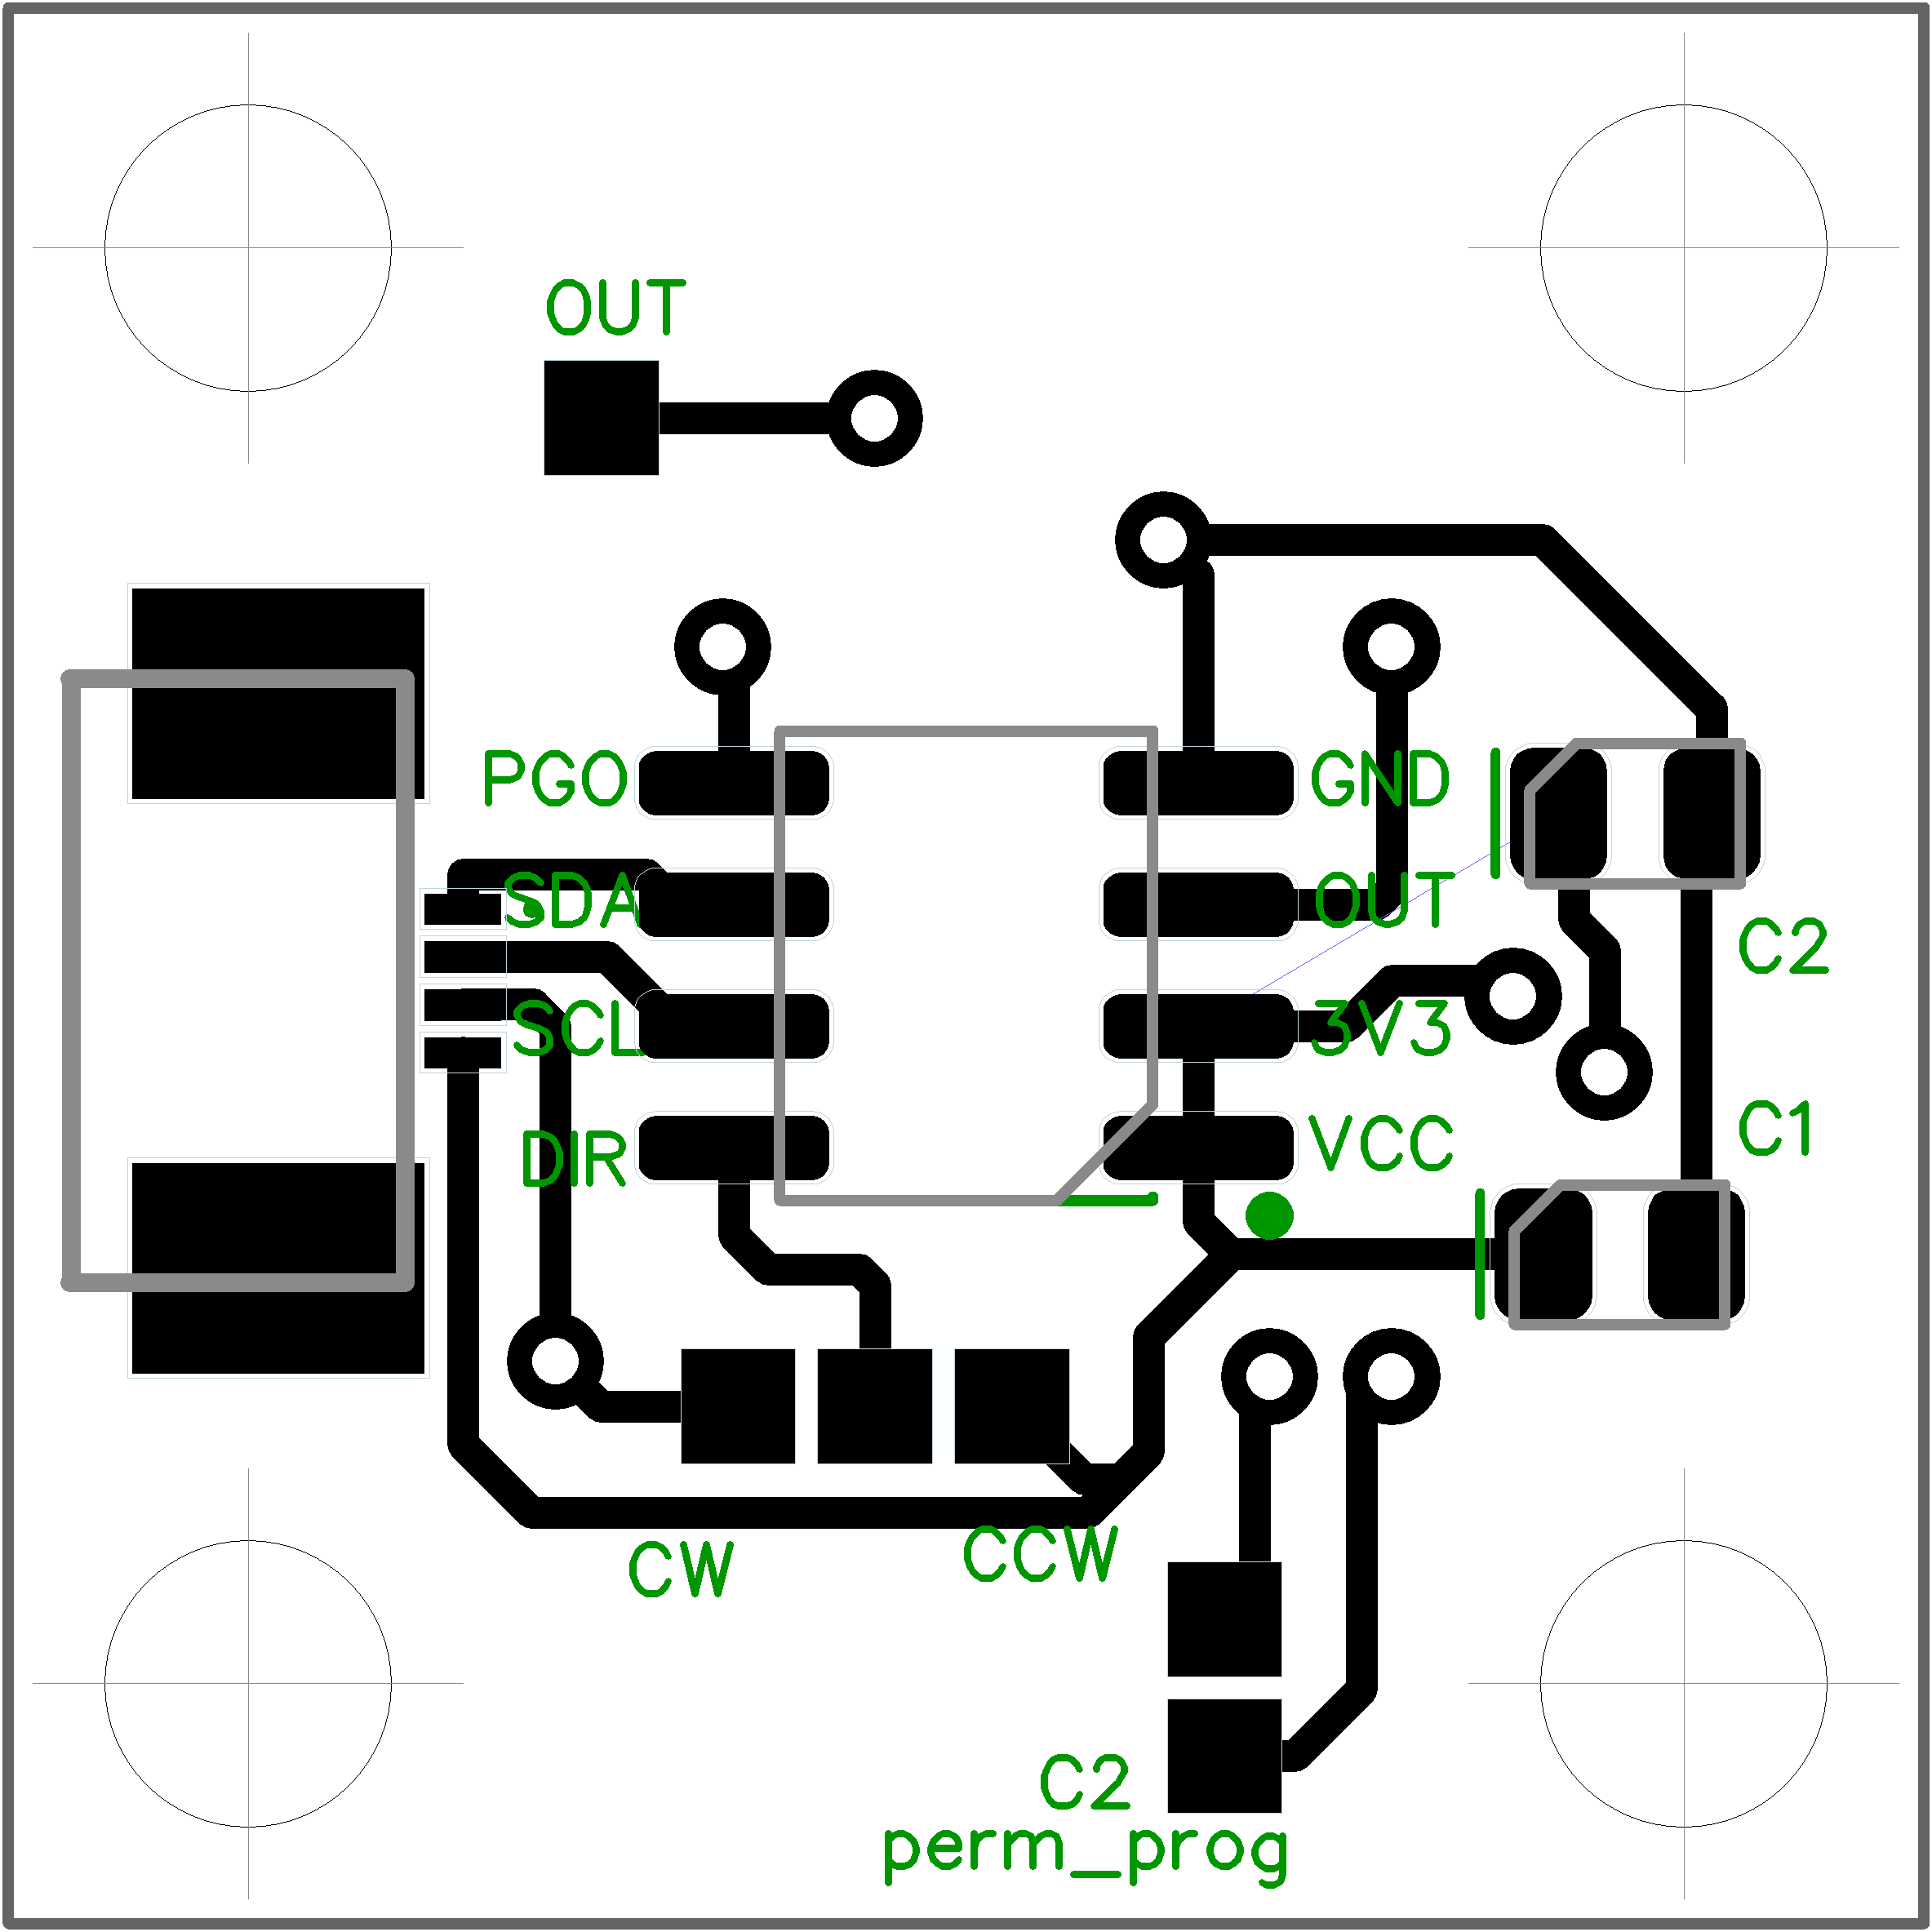
\includegraphics[width=7cm]{obr/breakoutTOP.png}}
	\hfill
	\subfigure[Spodná strana breakout boardu]{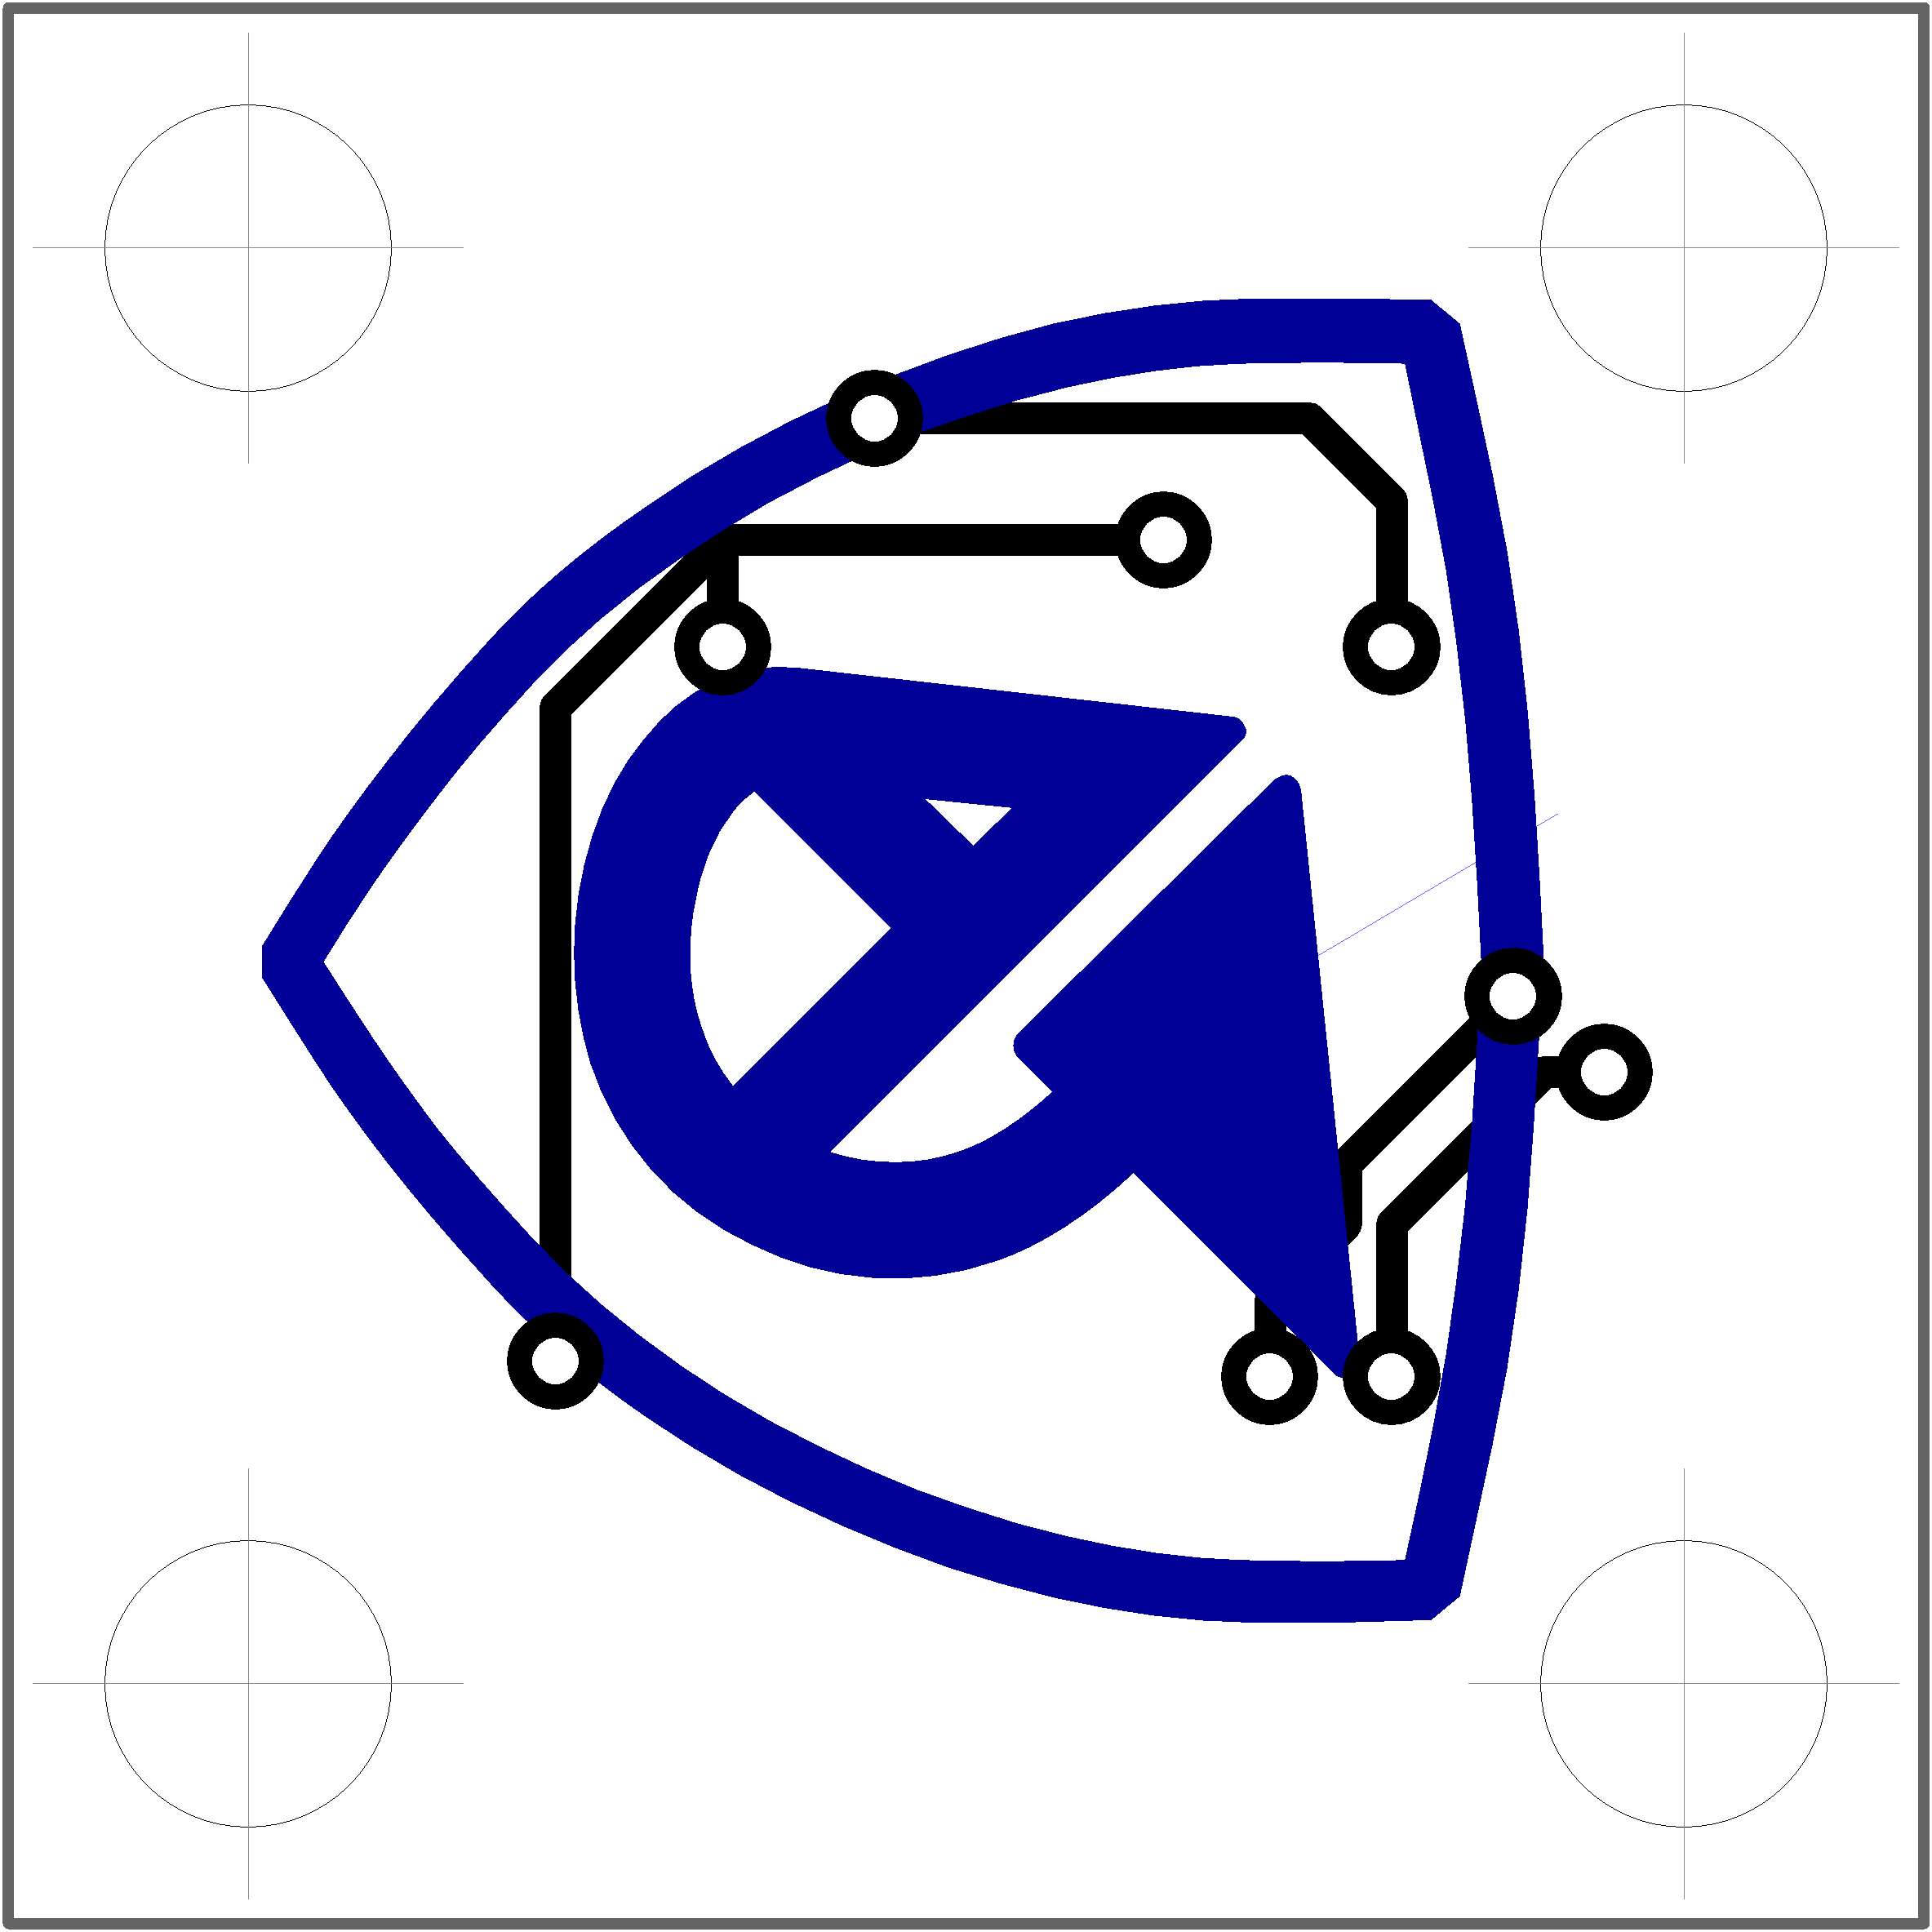
\includegraphics[width=7cm]{obr/breakoutbottom.png}}
	\hfill
	\caption{Vedlajšia doska AeroShieldu- breakout board}\label{OBRAZOK 2.6}
\end{figure}

Po zvolení optimálneho rozmiestnenia komponentov treba jednotlivé piny poprepájať vodivými cestami, ktoré nám nahrádzajú funkciu káblov. Máme možnosť zvoliť automatické rozmiestnenie ciest alebo ich manuálnu tvorbu. V našom prípade sme zvolili manuálnu tvorbu ciest, pretože ich vieme čo najlepšie optimalizovať. Ako je viditeľné aj na obr.\ref{OBRAZOK 2.4}.a, nie všetky cesty majú rovnakú šírku. Je to z toho titulu že niektorými cestami prúdi vyšší prúd a to až do 1A. V zásade sa používa pravidlo, čím vyšší prú preteka vodičom, tým väčšiu plochu prierezu by mal mať. Prúdy pretekajúce vodičmi tieto vodiče zahrievajú a pokiaľ je toto zahrievanie nadmerné, môže dôjsť k poškodeniu vodiča.  

Tvorba ciest má niekolko pravidiel, avšak najdôležitejšie z nich je že jednotlivé cesty ktoré v schéme zapojenia nie su prepojené, sa nemôžu križovať inak dôjde k ich vzájomnému vyskratovaniu. Z toho dôvodu treba niekedy cestu priviesť na druhú stranu dosky plošných spojov kde v jej pokračovaní neprekáža iná cesta. Na tento účel sa používajú vodivé diery, takzvané via, spájajúce obe strany dosky.

Pri výroby dosky sa taktiež myslelo na montáž držiaku kyvadla, pre ktoré boli vytvorené 4 diery na jeho následné prichytenie pomocou skrutiek. Finálna verzia hlavnej dosky je na obr.\ref{OBRAZOK 2.4}. Zhotovená bola aj menšia doska tzv. breakout board, slúžiaca na meranie uhlu kyvadla, ktorá je na obr.\ref{OBRAZOK 2.6}.



\begin{figure}
\centering
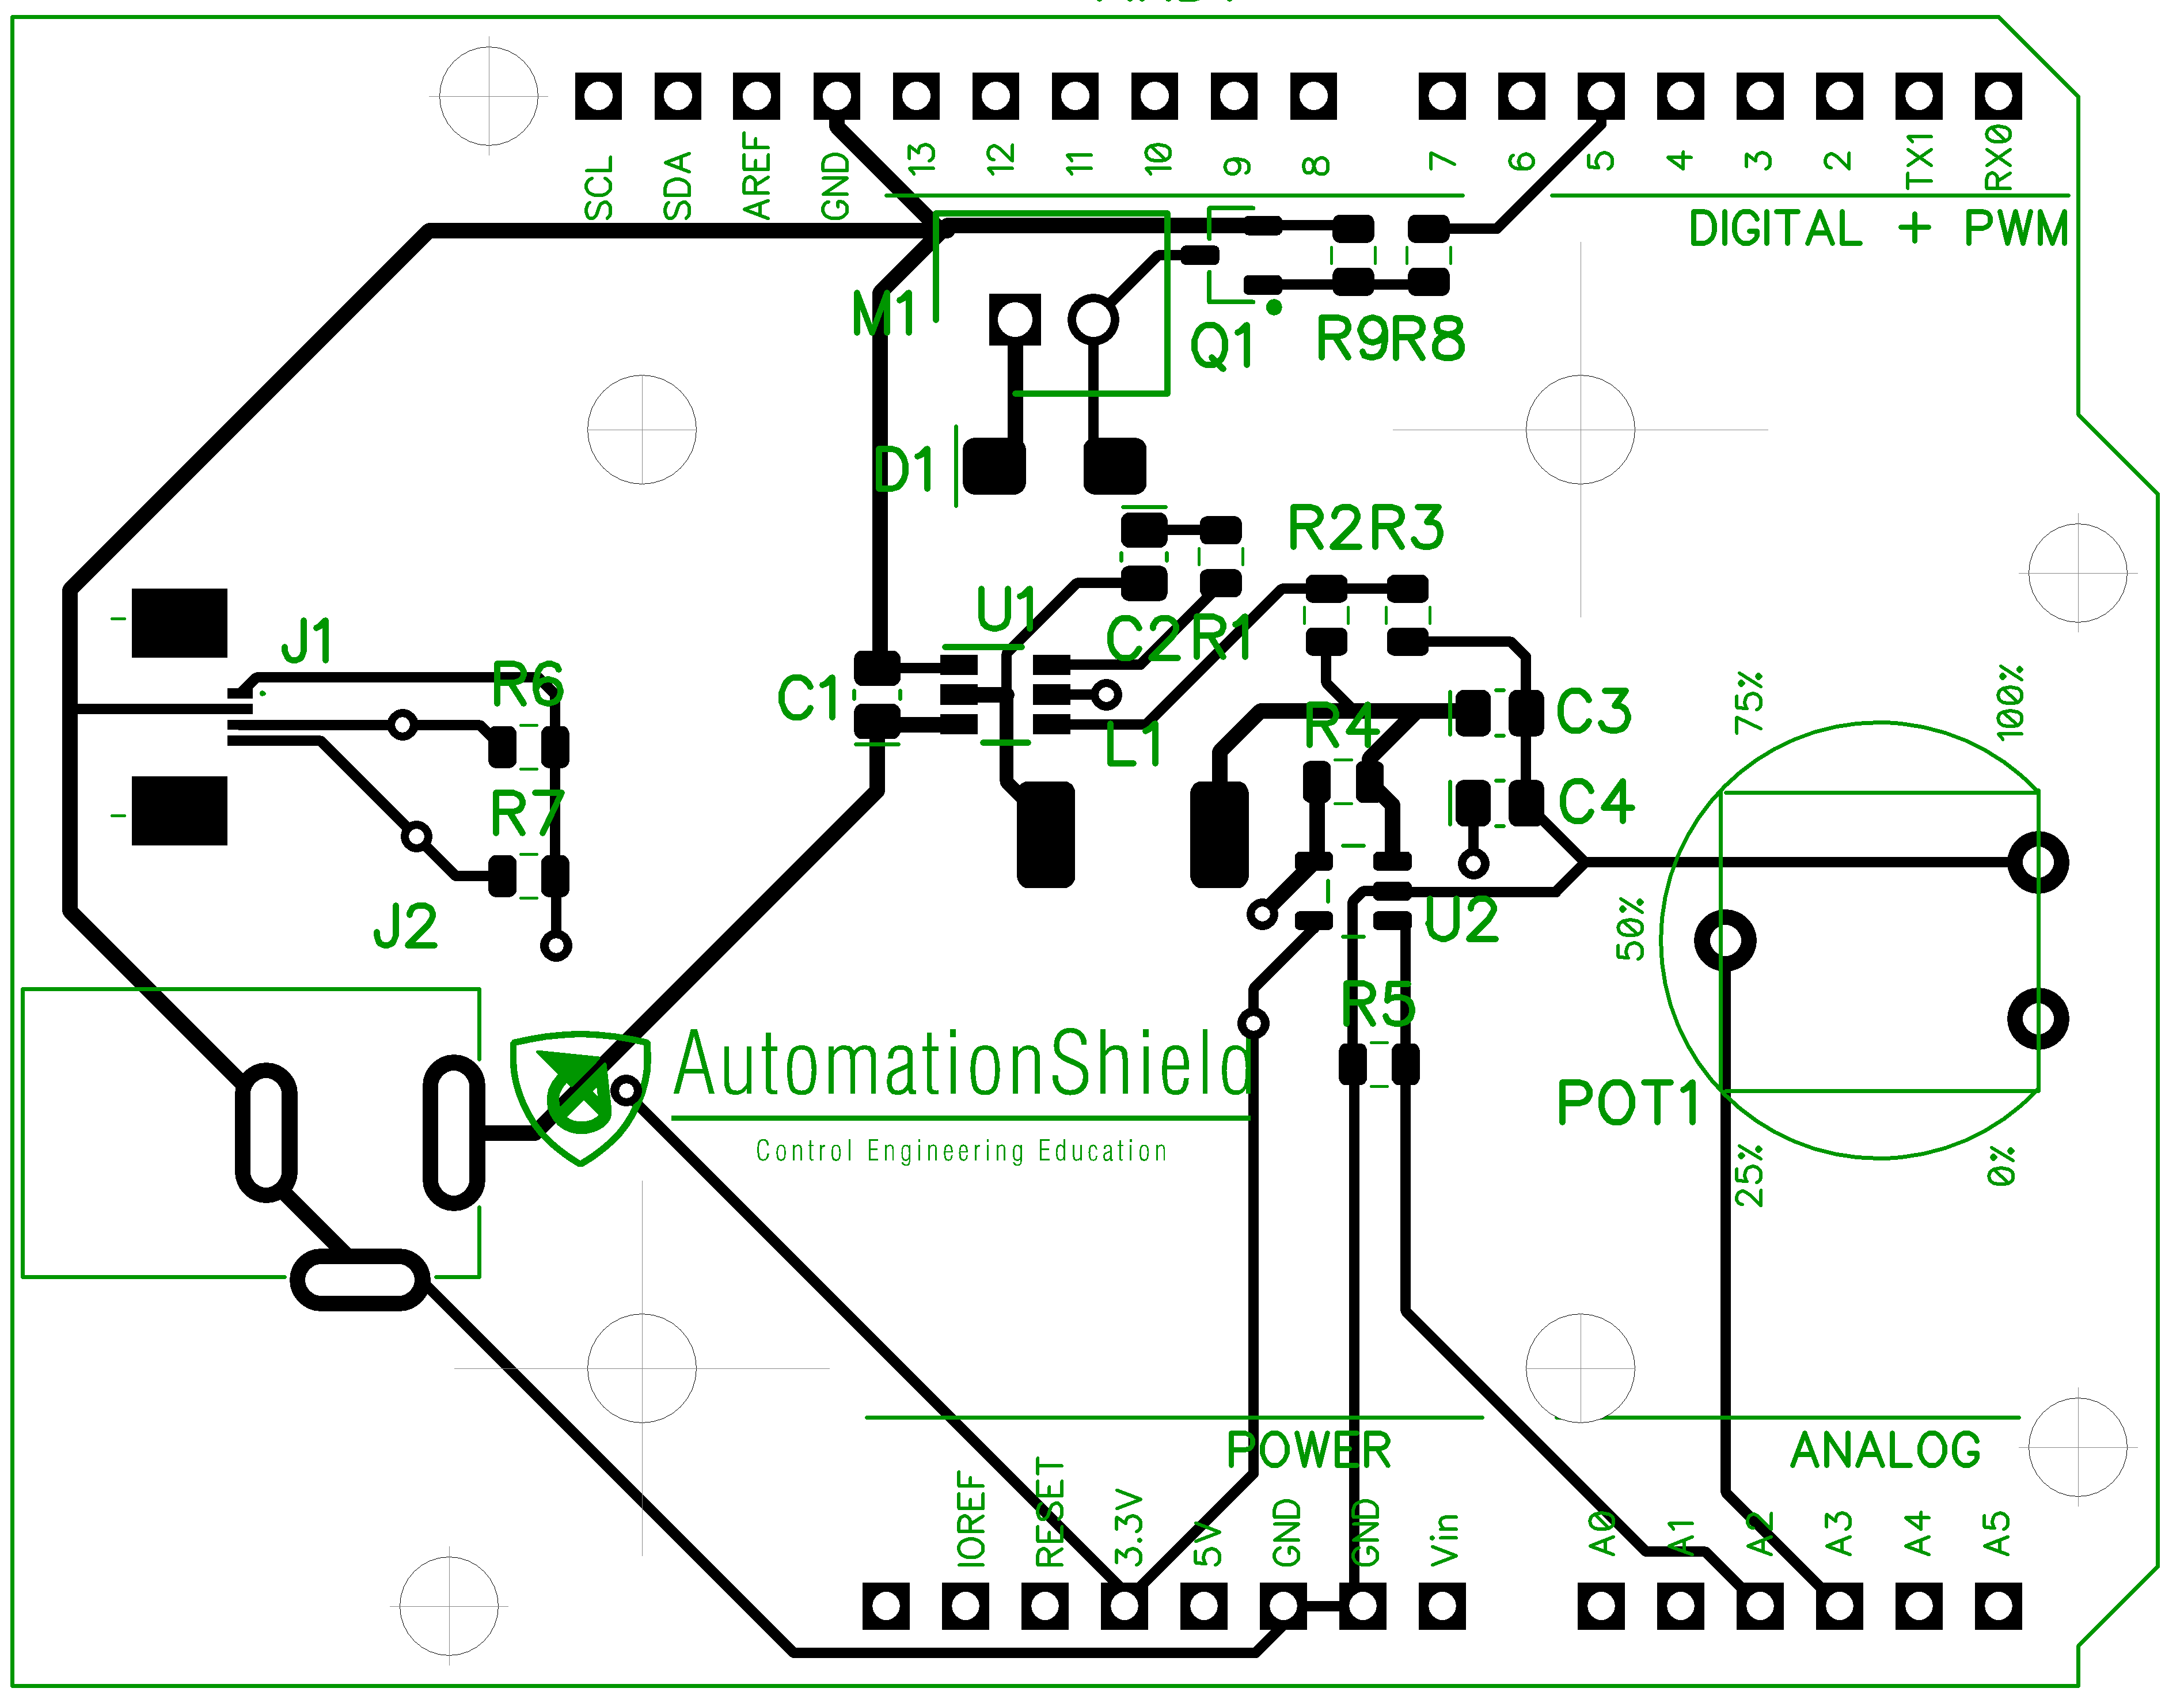
\includegraphics[width=8cm]{obr/AeroShieldTOP.png}

(a)

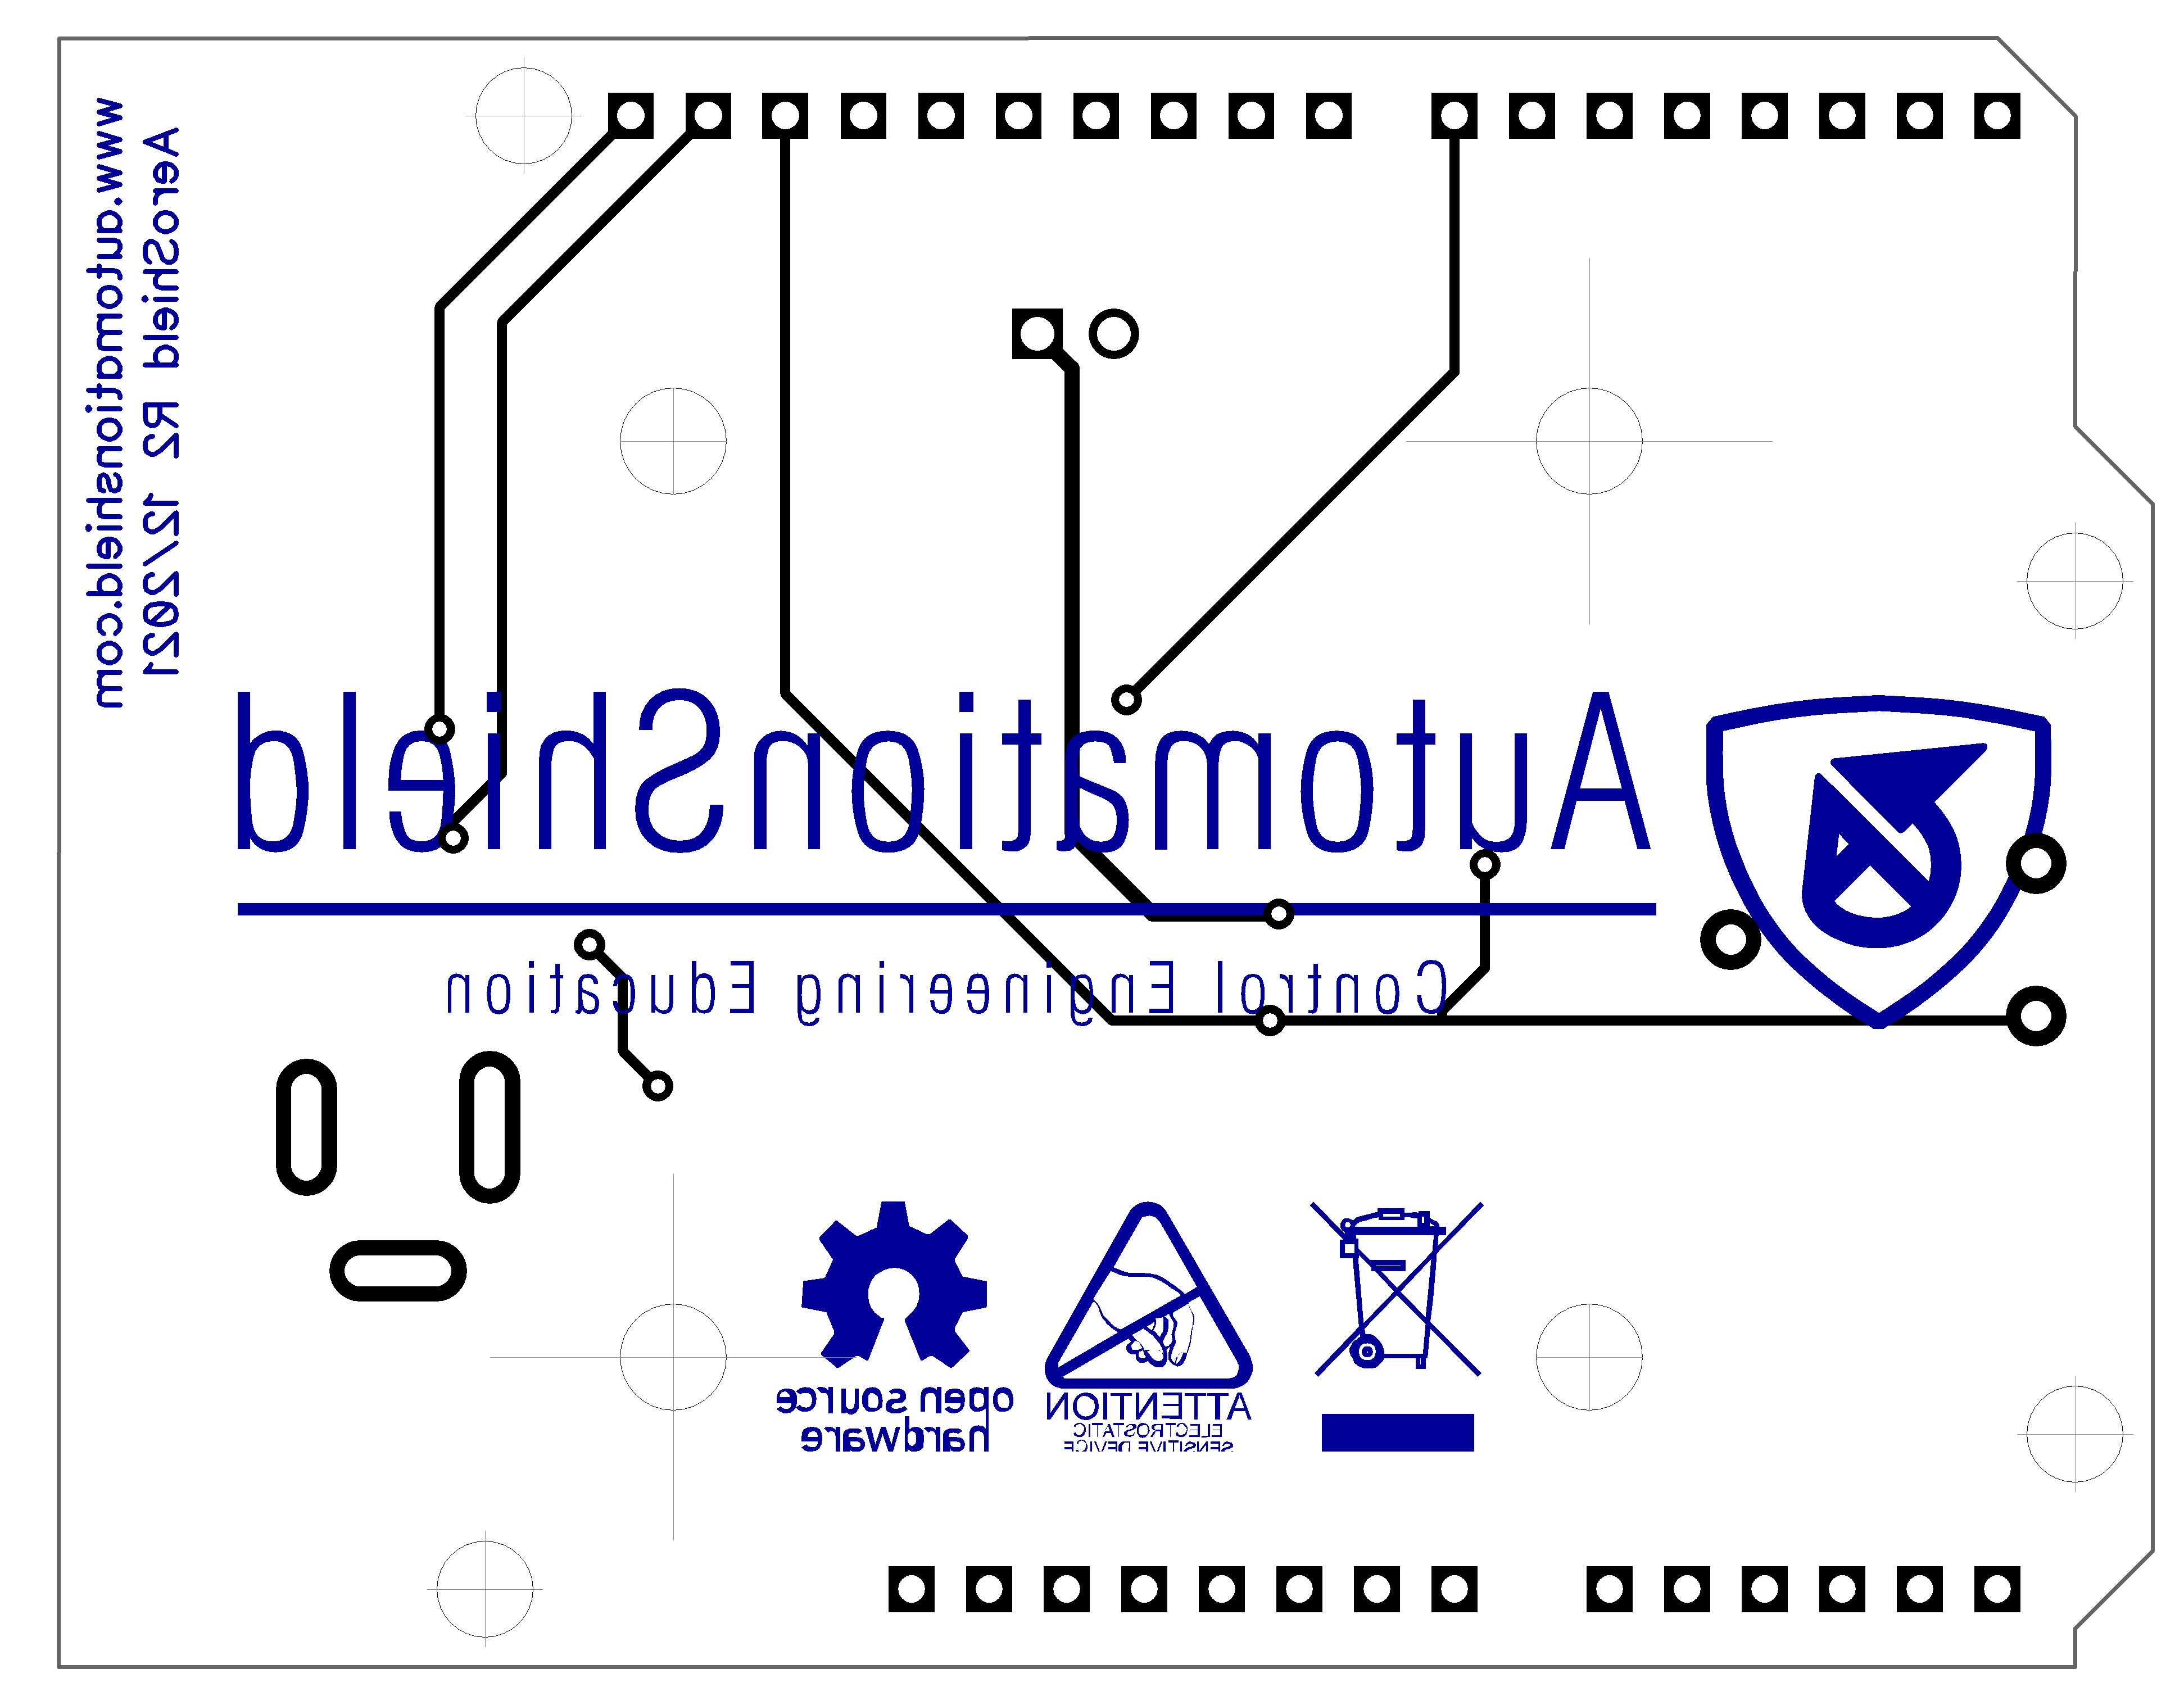
\includegraphics[width=8.5cm]{obr/AeroShieldBOTTOM.png}

(b)

\caption{(a) Vrchná strana AeroShieldu (b) Spodná strana AeroShieldu}
\label{OBRAZOK 2.4}
\end{figure}



Po finálnej kontrole zapojenia komponentov na doske plošných spojov môžeme tieto dosky uložiť do formátu gerber. Súbory typu gerber v sebe ukladajú presné zloženie finálnej dosky plošných spojov a to po jej jednotlivých vrstvách. Nachádza sa tu teda vrstva zobrazujúca vodivé cesty, vrstva pre konektory via, vrstva pre farebné popisy a mnoho ďalších. Pri tvorbe súboru máme veľa možností aké parametre jednotlivých vrstiev chceme zvoliť. Môžeme meniť hrúbky jednotlivých vrstiev, veľkostí dier a priestoru okolo dier, veľkosti konektorov via a iné. Gerber súbor ďalej posielame výrobcovi PCB dosiek kde si môžeme zvoliť dalšie parametre dosky, ako jej farbu, možnosti pájkovacích doštičiek, dokonca nám môže výrobca poslať už napájkovanú dosku, ktorá je tak hneď pripravená na použitie. Podobu finálnej dosky AeroShieldu môžeme vidieť na obr.\ref{OBRAZOK 2.7}.a a dosky breakout boardu na obr.\ref{OBRAZOK 2.7}.b.


\begin{figure}
\hfill
\subfigure[Hlavná doska AeroShieldu]{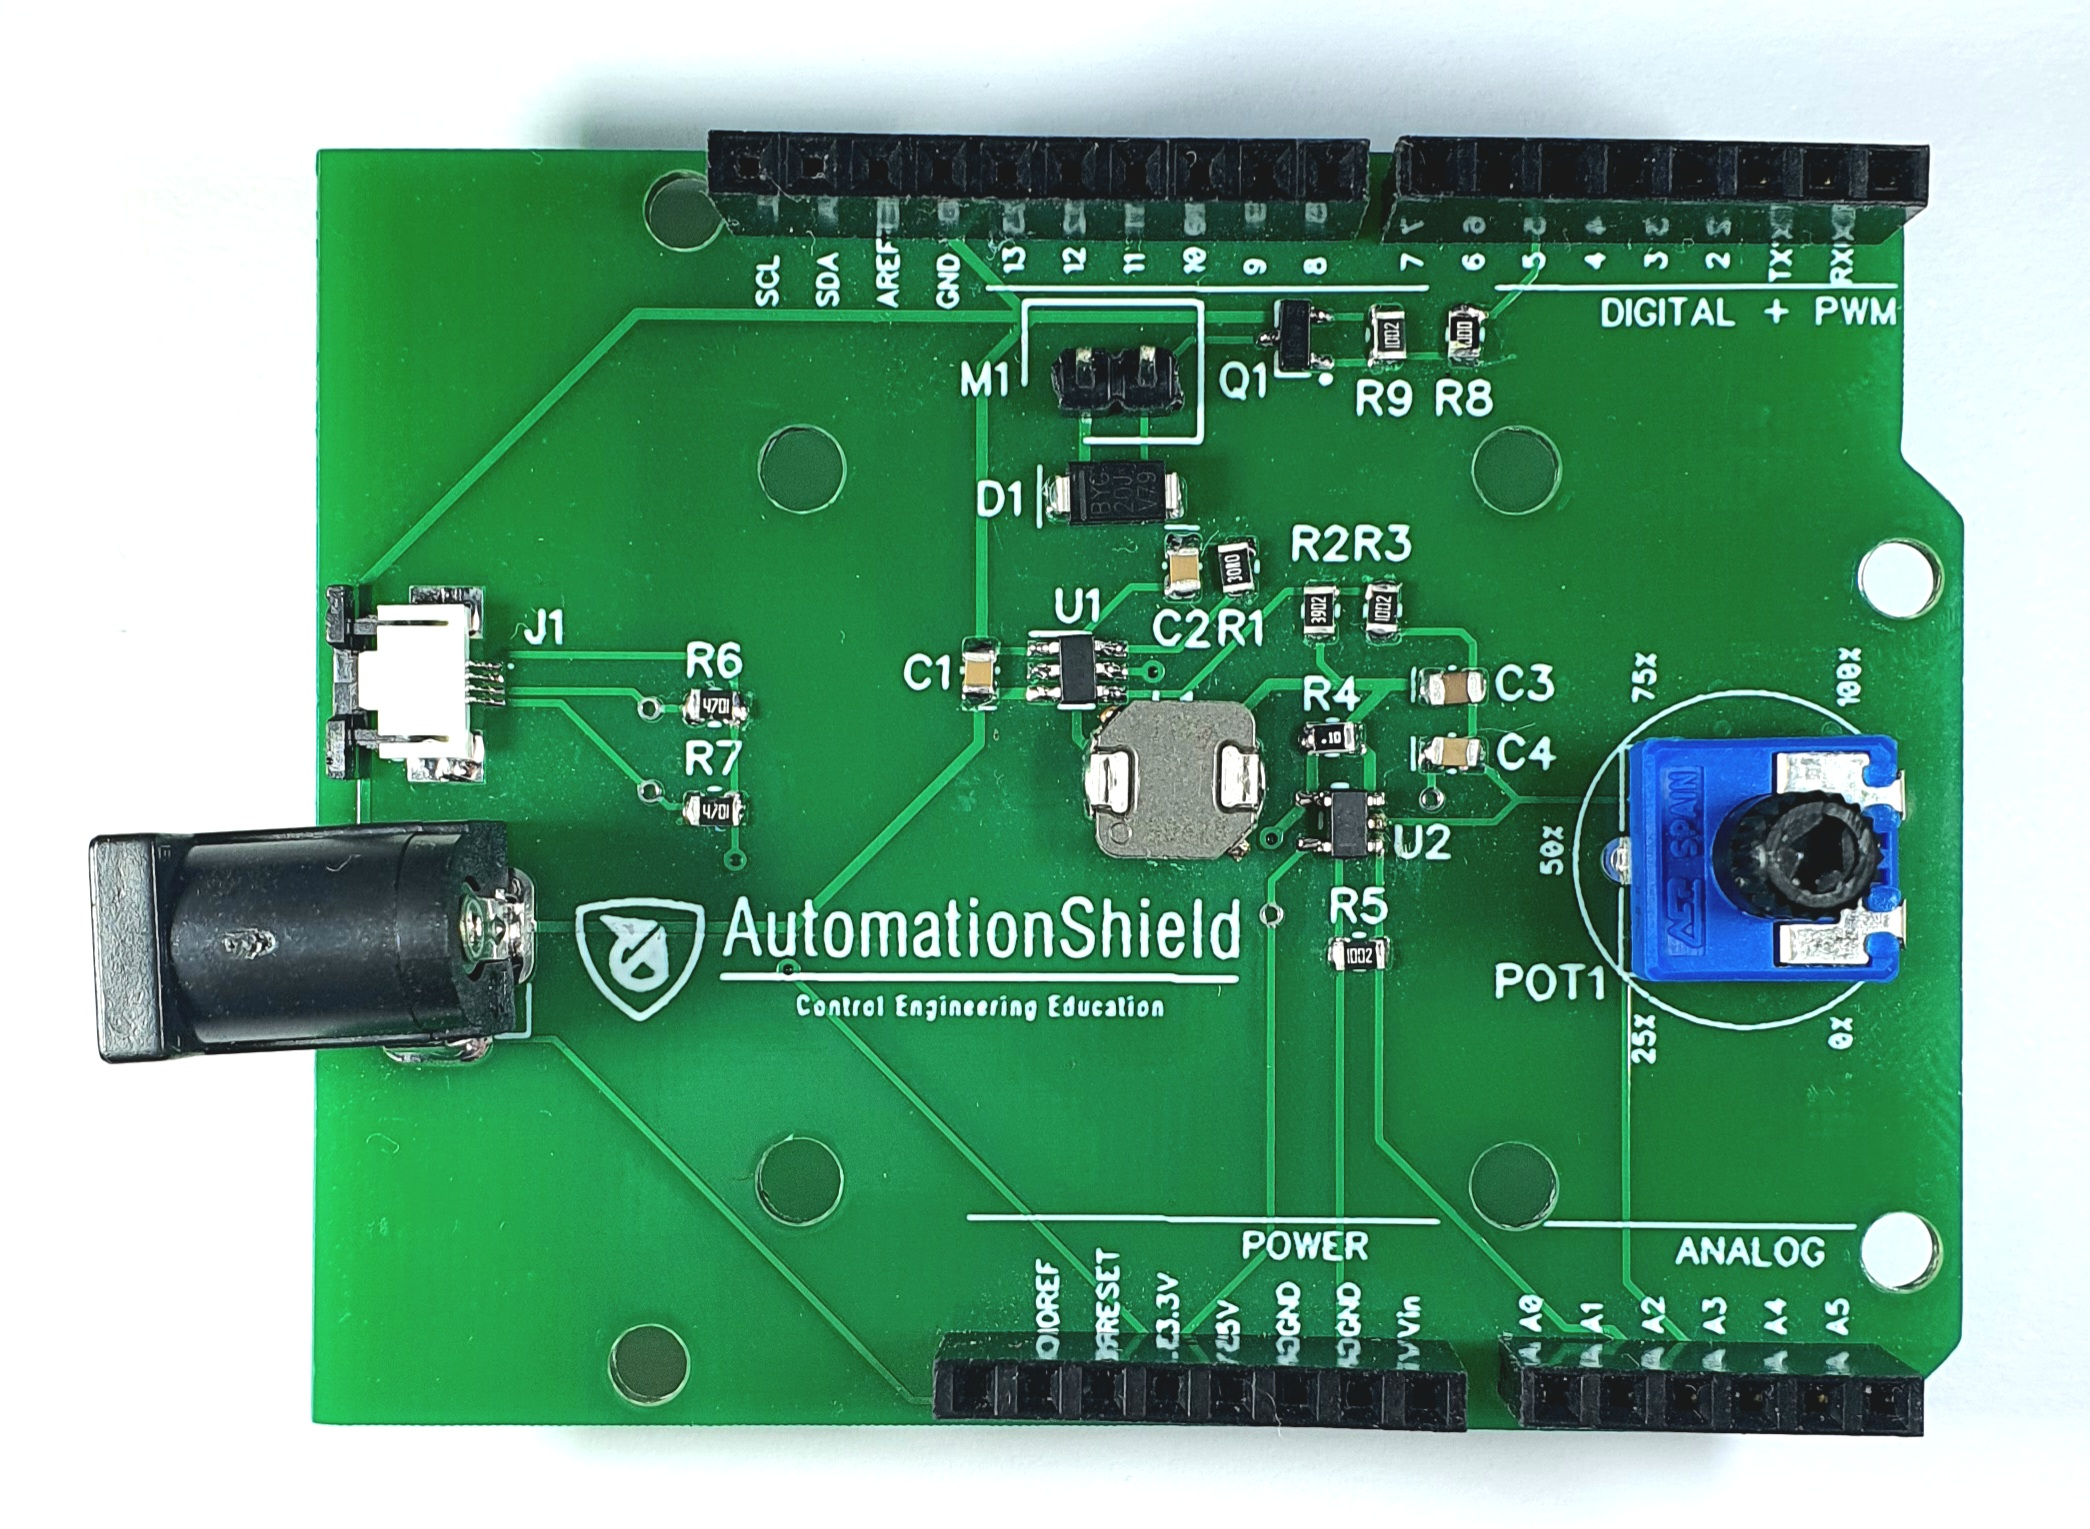
\includegraphics[width=9cm]{obr/AeroShield.jpg}}
\hfill
\subfigure[Vedľajšia doska AeroShieldu]{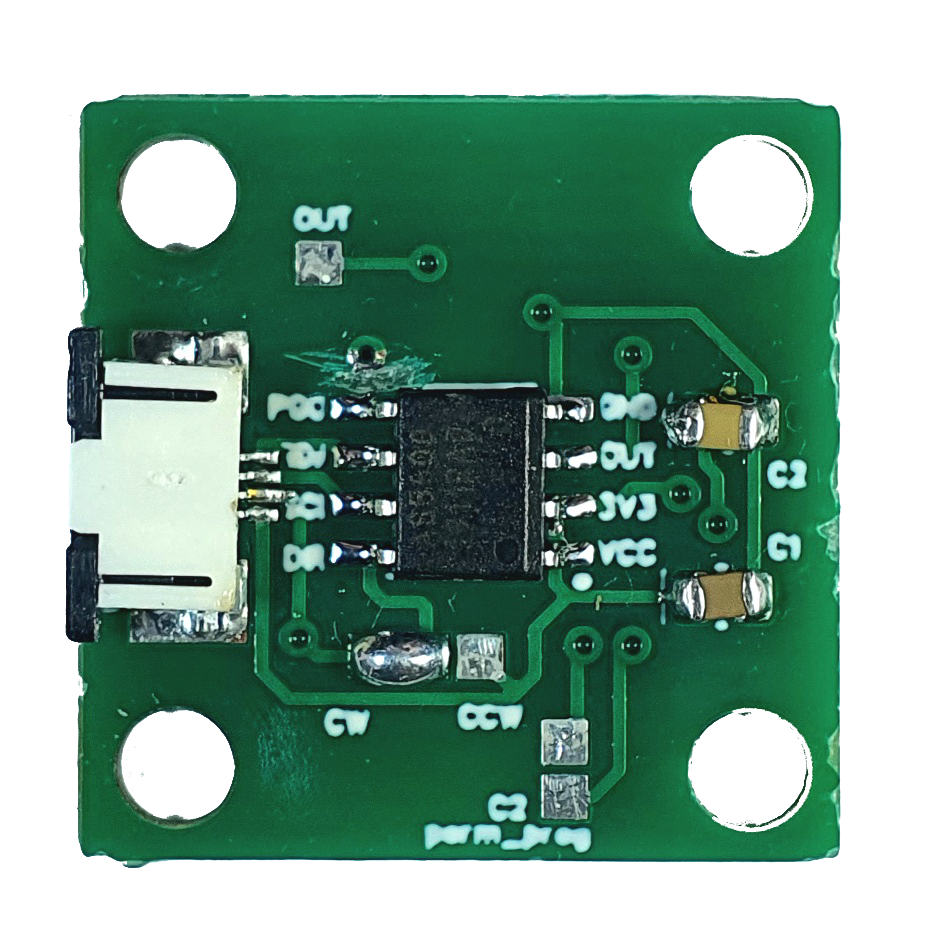
\includegraphics[width=6cm]{obr/fotoBreak.png}}
\hfill
\caption{Dosky plošných spojov AeroShieldu}\label{OBRAZOK 2.7}
\end{figure}

\subsection{Model držiaku kyvadla}

Tu ešte poviem čo to a designovaní držiaku pendulum 
